\chapter{Mathematical Review: Elliptic Curves, Pairings, and Interpolation}
\chaptermark{Mathematical Review 3}
\label{chap:math_3}

In this chapter we continue on to more advanced mathematics.
Understanding the information here is not required before reading
other parts of the document.
Even so, the more advanced parts of this document will require some familiarity
with these topics.

\section{Important Information}

\begin{itemize}
\item \Gls{publiccrypto}, such as the \gls{dhke},
    requires \glspl{cyclic group}.
    Many \glspl{cyclic group} may be constructed from \glspl{elliptic curve}
    with greater flexibility than the other \glspl{group}
    discussed in Chapter~\ref{sec:math_groups}
    or Example~\ref{example:math_field_p_more}.
\item \Glspl{bilinear} allow for many interesting possibilities;
    in particular, they allow for \glspl{signature}
    like BLS signatures~\cite{BLSSignatures}.
    More generally, they allow for \Gls{pairingcrypto}
    as discussed in Chapter~\ref{chap:pairing}.
\item \Gls{lagrange interpolation} is used in the secret sharing protocols
    in Chapter~\ref{chap:secret_sharing}.
\end{itemize}

\section{Elliptic Curves}
\label{sec:math_elliptic_curves}

\subsection{Why do we care about Elliptic Curves?}

\Glspl{elliptic curve} are fascinating and extremely useful in
\gls{number theory}.
We will give a brief introduction that will set the stage
for what we need in \gls{publiccrypto}.

We begin by noting \emph{why} we care about \glspl{elliptic curve}.
\Gls{publiccrypto} requires \glspl{group}
of various sizes and properties.
It turns out that there is a lot of freedom when constructing
specific \glspl{elliptic curve},
and it is easy to make many different kinds of \glspl{group}.
This freedom is what allows \glspl{elliptic curve} to be chosen
to have particular properties that are useful in \gls{publiccrypto}.

\subsection{Elliptic Curves are \emph{not} Ellipses}

First, we note that an \gls{elliptic curve} is \emph{not} an ellipse.
We recall that an ellipse over the reals has the form

\begin{equation}
    \parens{\frac{x}{a}}^{2} + \parens{\frac{y}{b}}^{2} = 1
\end{equation}

\noindent
for constants $a,b>0$ and $x,y\in\R$.
Figure~\ref{fig:ellipse_plot} shows an example of an ellipse.

\begin{figure}[t]
\centering
    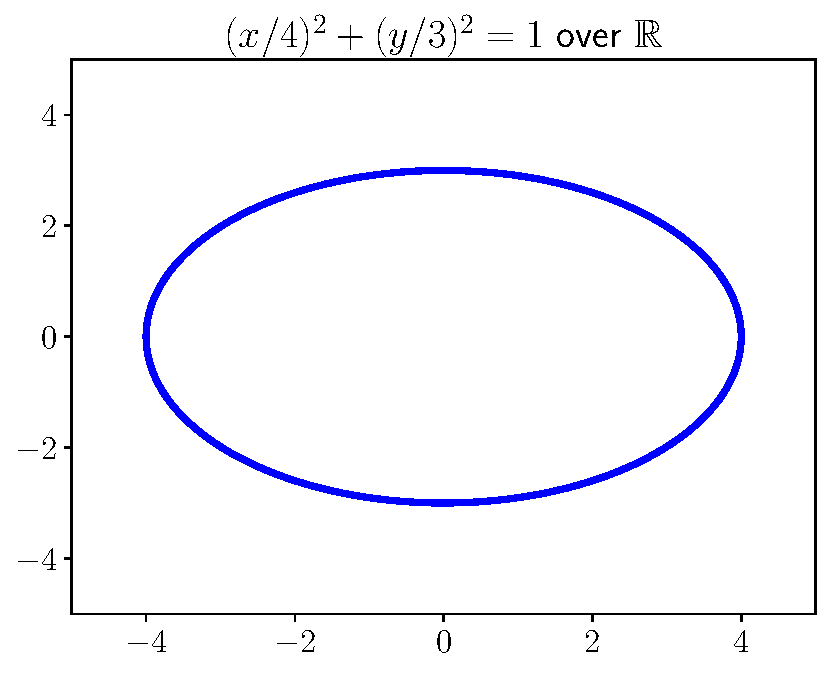
\includegraphics[width=10cm]{plots/ellipse/ellipse_reals_4_3.pdf}
    \caption[Plot of an ellipse over the reals]{Here
        is a plot of an ellipse over $\R$.
        Ellipses are \emph{not} \glspl{elliptic curve}.}
    \label{fig:ellipse_plot}
\end{figure}


Even though \glspl{elliptic curve} are not ellipses,
they are useful for jumping into our discussion of \glspl{elliptic curve}.
Ellipses describe a collection of points which satisfy a polynomial equation;
in this case, a particular quadratic equation.
Additionally, we have some notion of geometry by looking
at the points which satisfy the equation.
\Glspl{elliptic curve} arise in a similar manner but from a different polynomial
equation.

We will never mention ellipses again.

\subsection{Elliptic Curves over the Reals}

We will now look at some examples of \glspl{elliptic curve} over $\R$.
To do this, we will look at $\parens{x,y}\in\R^{2}$ which satisfy

\begin{equation}
    y^{2} = x^{3} + ax + b
    \label{eq:ec_reals}
\end{equation}

\noindent
for $a,b\in\R$.
Example plots can be found in Figures~\ref{fig:ec_real_plots_1}
and \ref{fig:ec_real_plots_2}.

\begin{figure}[p]
\centering
    \begin{subfigure}[t]{0.45\textwidth}
    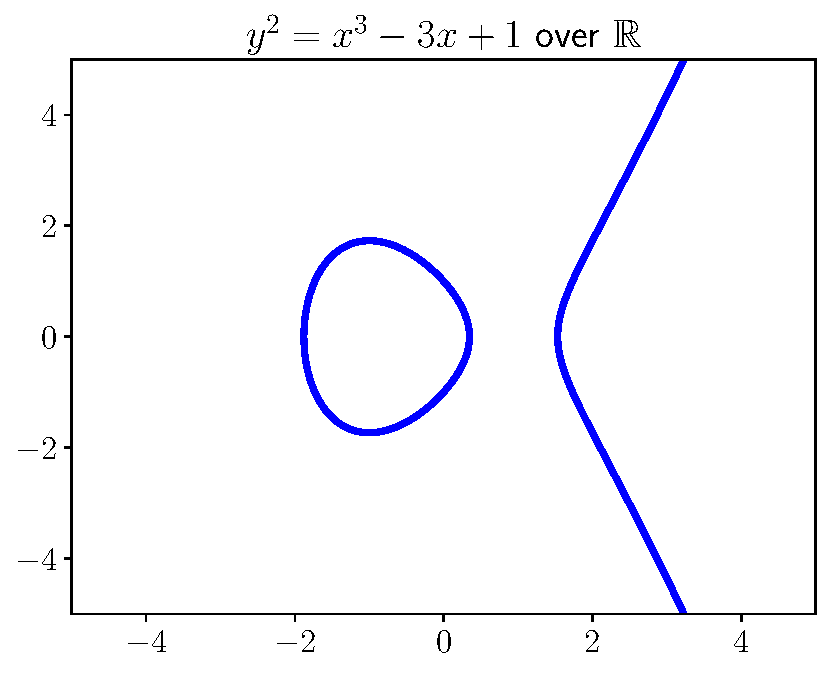
\includegraphics[width=\textwidth]{plots/ec_reals/ec_reals_n3_1.pdf}
    \end{subfigure}
    \begin{subfigure}[t]{0.45\textwidth}
    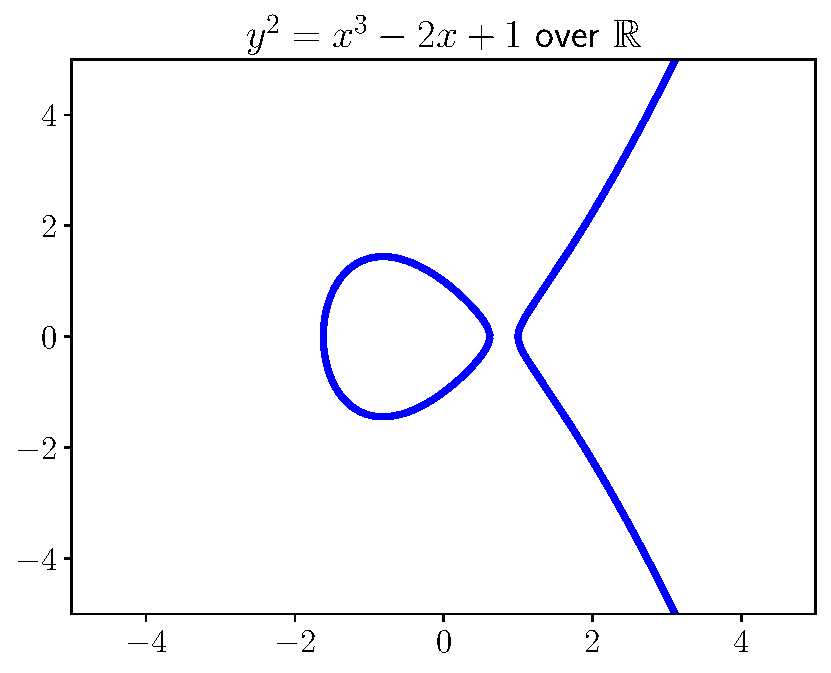
\includegraphics[width=\textwidth]{plots/ec_reals/ec_reals_n2_1.pdf}
    \end{subfigure}

    \begin{subfigure}[t]{0.45\textwidth}
    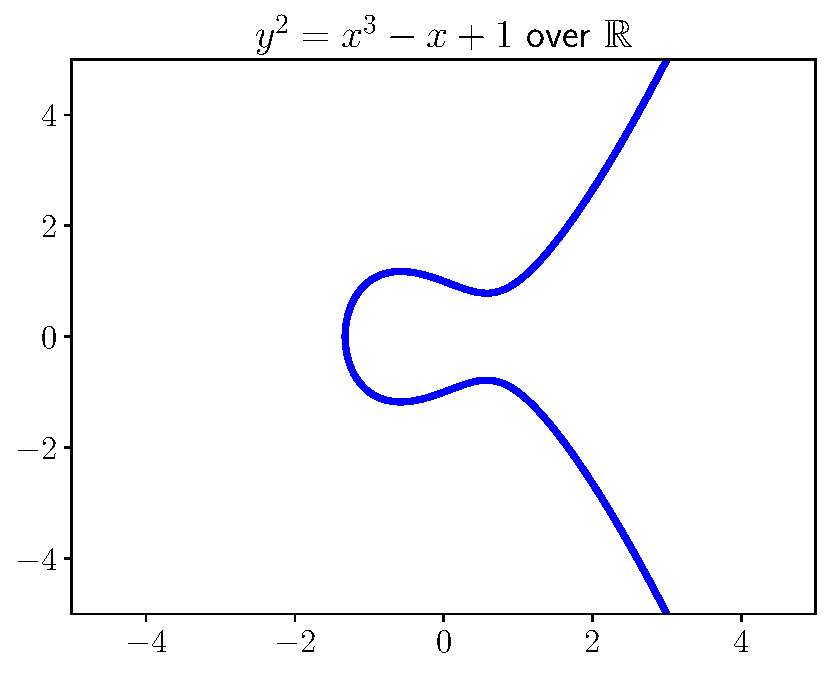
\includegraphics[width=\textwidth]{plots/ec_reals/ec_reals_n1_1.pdf}
    \end{subfigure}
    \begin{subfigure}[t]{0.45\textwidth}
    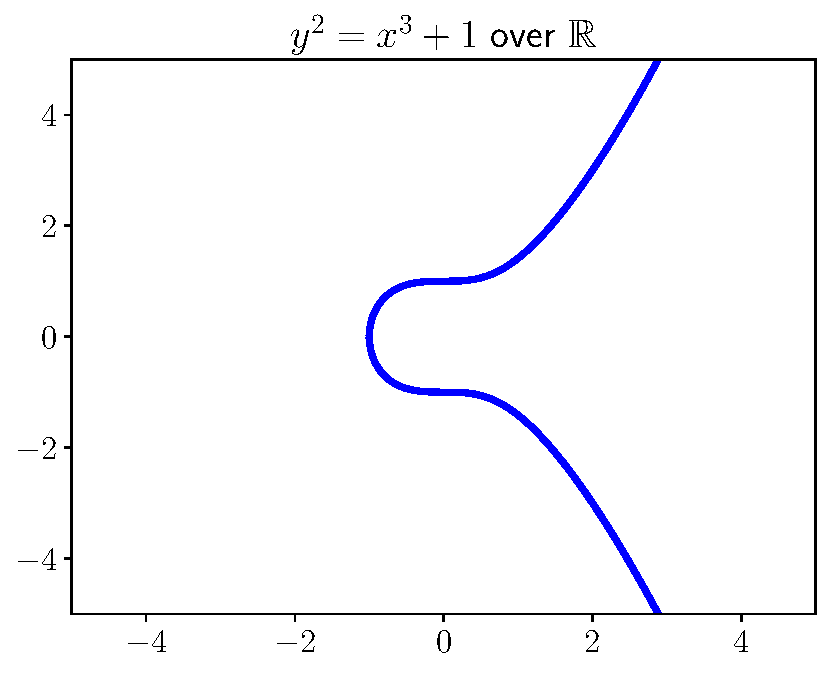
\includegraphics[width=\textwidth]{plots/ec_reals/ec_reals_0_1.pdf}
    \end{subfigure}

    \begin{subfigure}[t]{0.45\textwidth}
    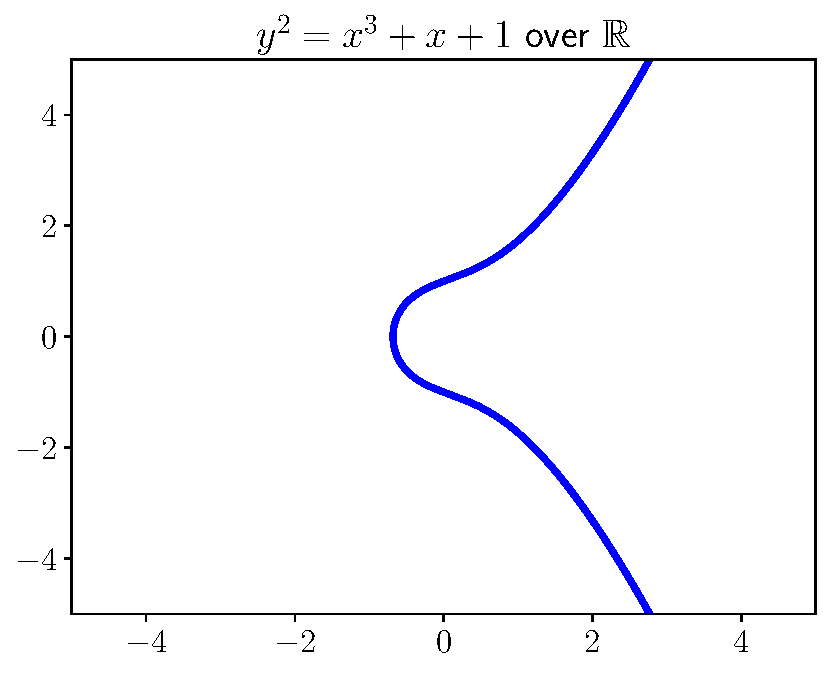
\includegraphics[width=\textwidth]{plots/ec_reals/ec_reals_1_1.pdf}
    \end{subfigure}
    \begin{subfigure}[t]{0.45\textwidth}
    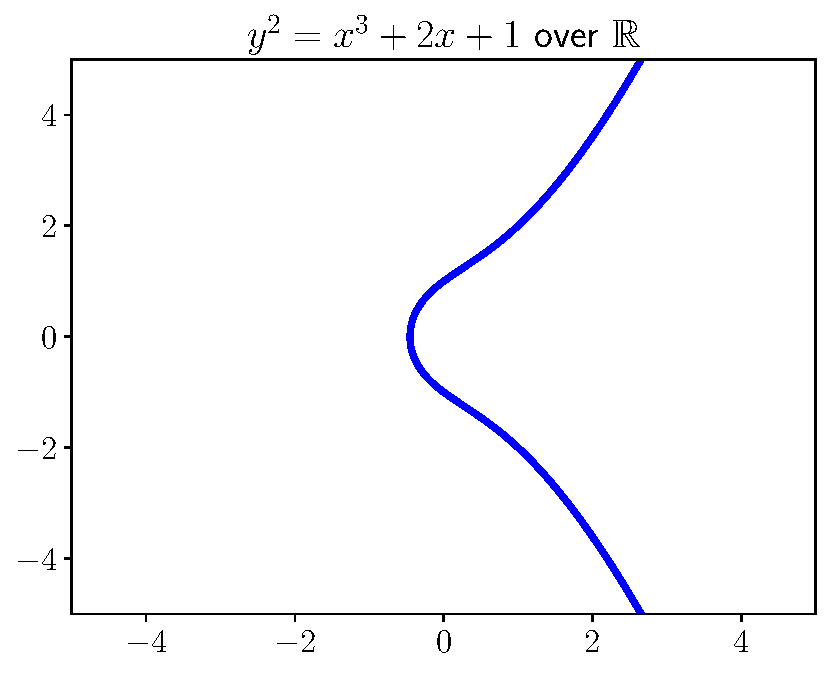
\includegraphics[width=\textwidth]{plots/ec_reals/ec_reals_2_1.pdf}
    \end{subfigure}
    \caption[Plots of elliptic curves over the reals 1]{Here
        are plots of \glspl{elliptic curve} over $\R$.
        The $\parens{x,y}$ points satisfy the equation
        $y^{2} = x^{3} + ax + b$;
        we vary $a$ and hold $b$ constant.}
    \label{fig:ec_real_plots_1}
\end{figure}

\begin{figure}[p]
\centering
    \begin{subfigure}[t]{0.45\textwidth}
    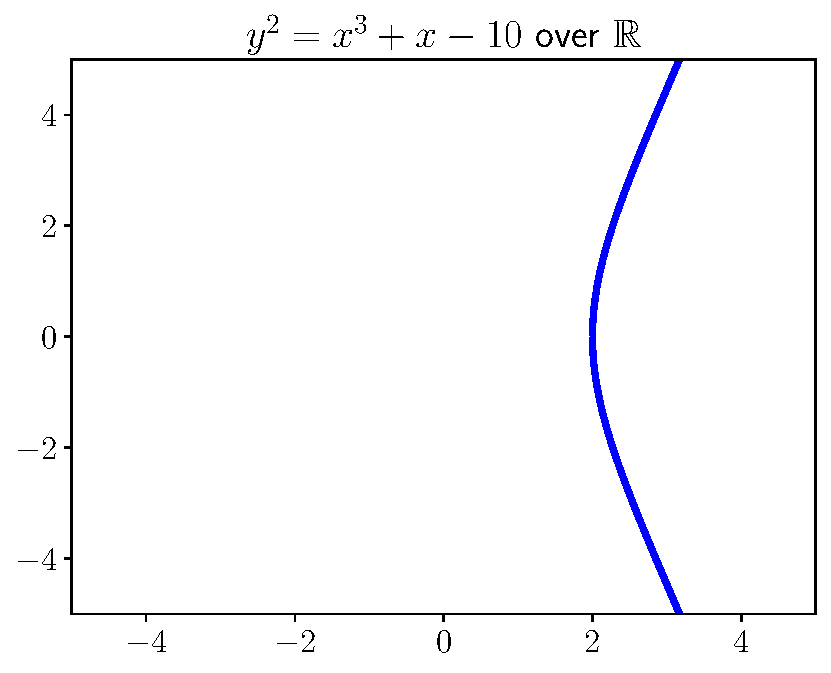
\includegraphics[width=\textwidth]{plots/ec_reals/ec_reals_1_n10.pdf}
    \end{subfigure}
    \begin{subfigure}[t]{0.45\textwidth}
    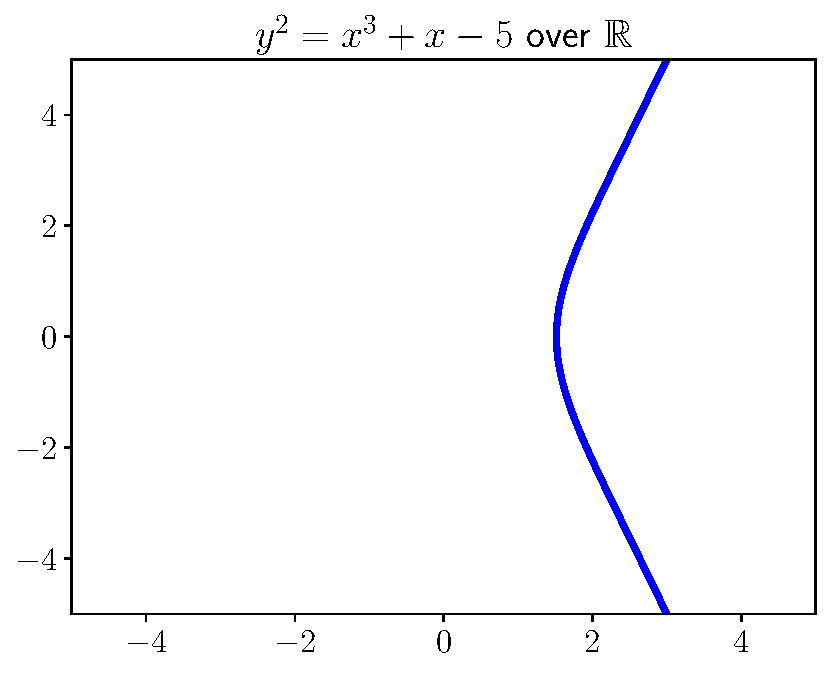
\includegraphics[width=\textwidth]{plots/ec_reals/ec_reals_1_n5.pdf}
    \end{subfigure}

    \begin{subfigure}[t]{0.45\textwidth}
    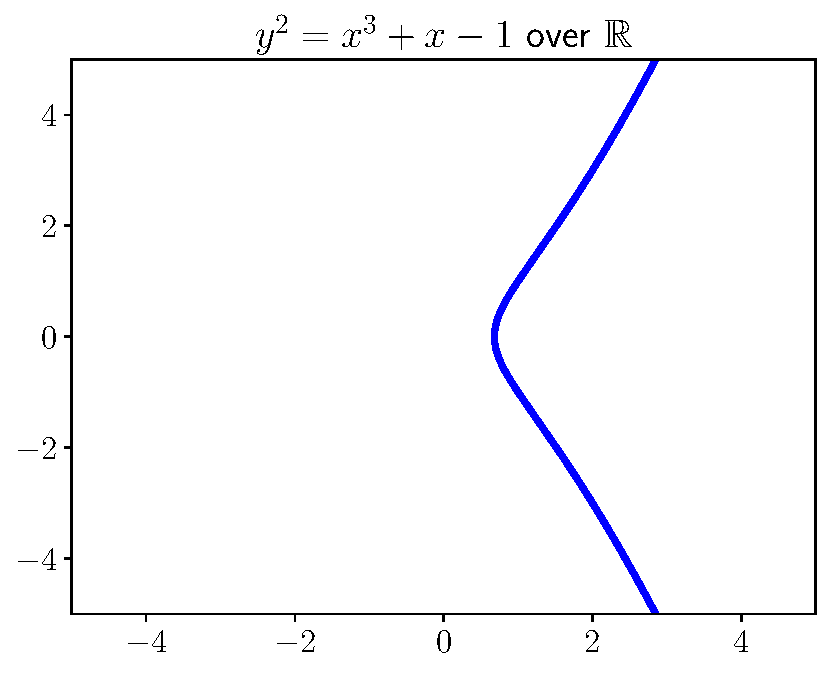
\includegraphics[width=\textwidth]{plots/ec_reals/ec_reals_1_n1.pdf}
    \end{subfigure}
    \begin{subfigure}[t]{0.45\textwidth}
    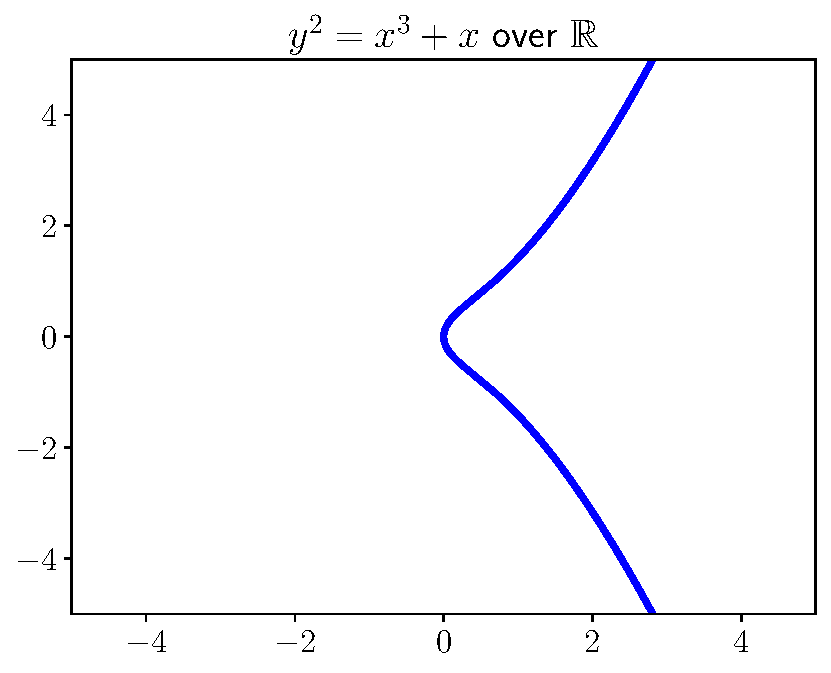
\includegraphics[width=\textwidth]{plots/ec_reals/ec_reals_1_0.pdf}
    \end{subfigure}

    \begin{subfigure}[t]{0.45\textwidth}
    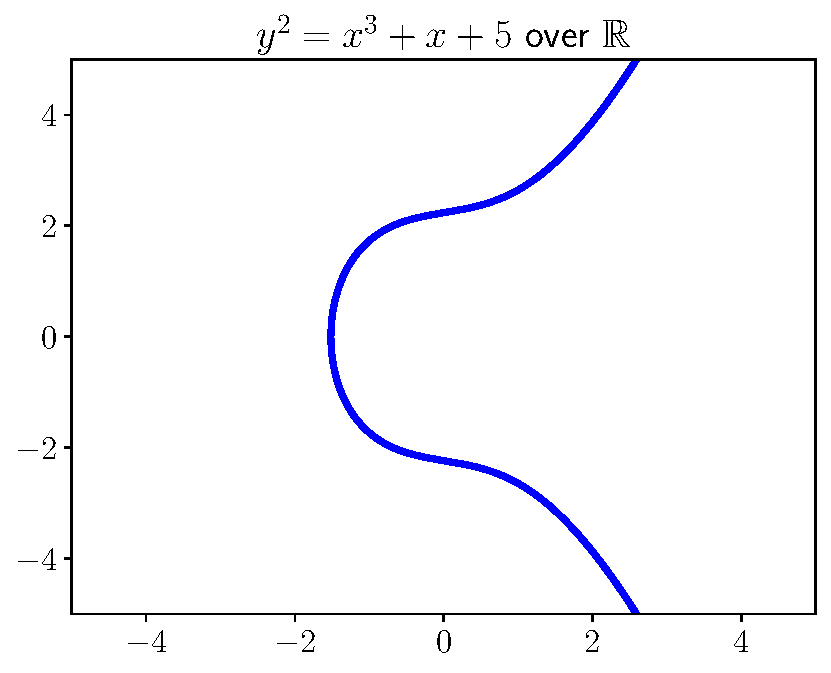
\includegraphics[width=\textwidth]{plots/ec_reals/ec_reals_1_5.pdf}
    \end{subfigure}
    \begin{subfigure}[t]{0.45\textwidth}
    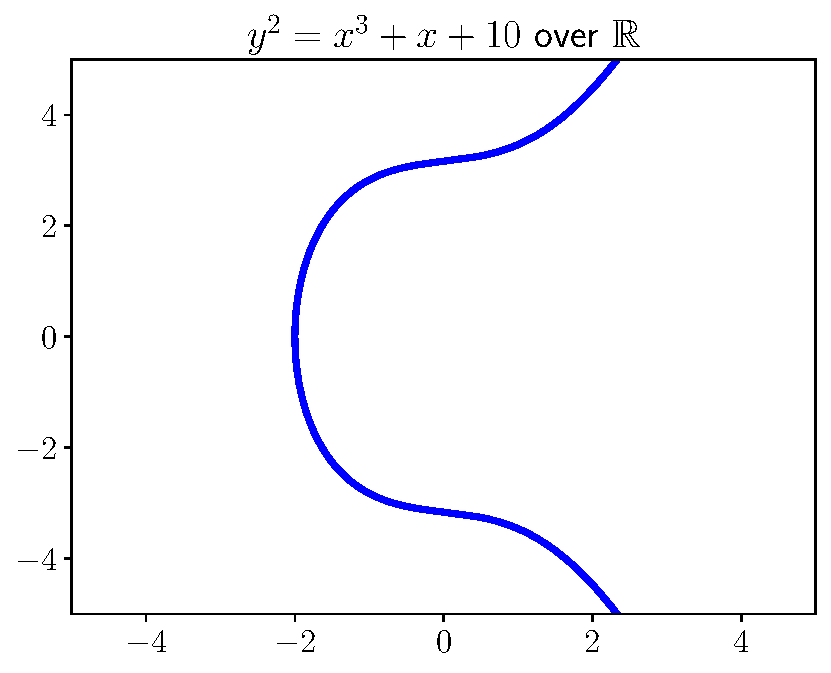
\includegraphics[width=\textwidth]{plots/ec_reals/ec_reals_1_10.pdf}
    \end{subfigure}
    \caption[Plots of elliptic curves over the reals 2]{Here
        are additional plots of \glspl{elliptic curve} over $\R$.
        The $\parens{x,y}$ points satisfy the equation
        $y^{2} = x^{3} + ax + b$;
        we vary $b$ and hold $a$ constant.}
    \label{fig:ec_real_plots_2}
\end{figure}


First, we notice the symmetry about the $x$-axis.
We expect this symmetry because we have
$y^{2} = \cdots$ in Eq.~\eqref{eq:ec_reals}.
Furthermore, we note that by changing $a$ and $b$, we change characteristics
of the curve.
In Figure~\ref{fig:ec_real_plots_1} we vary $a$;
in Figure~\ref{fig:ec_real_plots_2} we vary $b$.

\subsection{Elliptic Curve Addition}
\label{ssec:math_elliptic_addition}

We previously stated that \glspl{elliptic curve} give more freedom
to construct \glspl{group}.
At this point, it is not clear what the \gls{group} structure is,
as we have just seen the equation defining the curve
and looked at some plots.

We now define addition on points of \glspl{elliptic curve}.
As before, we will be looking at points $\parens{x,y}$ which satisfy

\begin{equation}
    y^{2} = x^{3} + ax + b.
    \label{eq:ec_addition}
\end{equation}

\noindent
We also include a special point $\mathcal{O}$;
this point is the additive identity on the \gls{elliptic curve}.
Thus, for any point $P$ on the \gls{elliptic curve},
we have

\begin{equation}
    \mathcal{O} + P = P.
\end{equation}

We suppose that $P = \parens{x_{1},y_{1}}$
and $Q = \parens{x_{2},y_{2}}$ with $P\ne\mathcal{O}$
and $Q\ne\mathcal{O}$;
that is, $P$ and $Q$ are points on the \gls{elliptic curve} which
are not the identity element.
We want to compute $R$ such that

\begin{equation}
    P + Q = R.
\end{equation}

\noindent
We have a few different cases to consider:

\begin{itemize}
\item Case 1: $x_{1}\ne x_{2}$ and $y_{1}\ne y_{2}$

This the general case.
We set

\begin{align}
    s &\mathDef{} \frac{y_{2}-y_{1}}{x_{2}-x_{1}} \nonumber\\
    x_{3} &\mathDef{} s^{2} - x_{1} - x_{2} \nonumber\\
    y_{3} &\mathDef{} s\parens{x_{1} - x_{3}} - y_{1}.
\end{align}

\noindent
In this case, we set

\begin{equation}
    R \mathDef{} \parens{x_{3},y_{3}}.
\end{equation}

\item Case 2: $x_{1} = x_{2}$ and $y_{1}\ne y_{2}$

In this case, we have $Q = -P$, so

\begin{equation}
    R \mathDef{} \mathcal{O}.
\end{equation}

\item Case 3: $x_{1} = x_{2}$ and $y_{1} = y_{2}$

In this case, we need to add a point to itself;
this is also called \emph{point doubling},
and we want to compute $P + P = R$.
We set

\begin{align}
    s &\mathDef{} \frac{3x_{1}^{2} + a}{2y_{1}} \nonumber\\
    x_{3} &\mathDef{} s^{2} - 2x_{1} \nonumber\\
    y_{3} &\mathDef{} s\parens{x_{1} - x_{3}} - y_{1}.
\end{align}

\noindent
In this case, we set

\begin{equation}
    R \mathDef{} \parens{x_{3},y_{3}}.
\end{equation}
\end{itemize}

\noindent
This, when including addition by the identity element,
is the entire addition formula;
one reference is \cite[Proposition~9.70]{IntroModernCrypto}.
Although we have not shown it, \glspl{elliptic curve}
form \glspl{abelian group};
this means that

\begin{equation}
    P + Q = Q + P
\end{equation}

\noindent
for all points $P$ and $Q$.

As mentioned above, if we have $P = \parens{x,y}$,
the additive inverse $-P$ satisfies

\begin{equation}
    -P \mathDef{} \parens{x,-y}.
\end{equation}

\noindent
Naturally, we have

\begin{equation}
    P + \parens{-P} = \mathcal{O}.
\end{equation}

The addition law described here depends on the particular form
of \gls{elliptic curve}.
Additional types of \glspl{elliptic curve} are discussed below,
and the addition formula described here does not always apply.
In fact, due to the nature of the addition formula
(involving conditional checks and different paths for different points),
certain \gls{ecc} (ECC) algorithms specifically
choose a different form of \gls{elliptic curve}.
The branch logic required to implement the above addition formula
will leak secret information if it is not
carefully implemented~\cite{brumley2011remote}.

Plots for elliptic curve addition in
Examples~\ref{example:ec_real_addition_1}
and \ref{example:ec_real_addition_2}
can be found in Figure~\ref{fig:ec_real_plots_addition}.

\begin{figure}[p]
\centering
    \begin{subfigure}[t]{\textwidth}
        \centering
    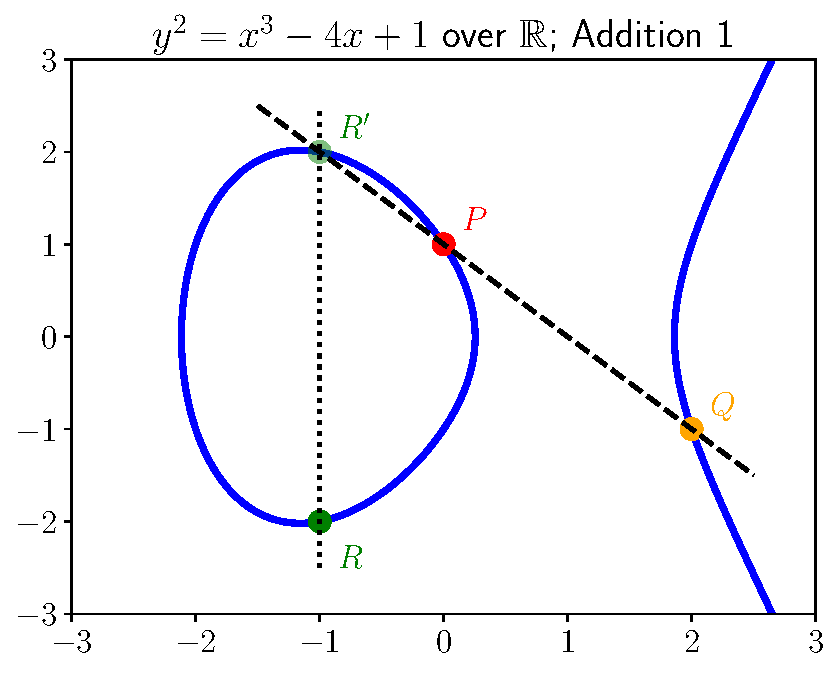
\includegraphics[width=0.70\textwidth]{plots/ec_reals/ec_reals_addition_1.pdf}
    \caption{Plot of elliptic curve addition over $\R$ for
        Example~\ref{example:ec_real_addition_1};
        this is an example of adding distinct points.
        We have
        $\textcolor{red}{P} + \textcolor{orange}{Q} =
        \textcolor[rgb]{0,0.33,0}{R}$.
        This figure shows
        $\textcolor{red}{\parens{0,1}} + \textcolor{orange}{\parens{2,-1}}
        = \textcolor[rgb]{0,0.33,0}{\parens{-1,-2}}$.}
    \label{fig:ec_real_plots_addition_1}
    \end{subfigure}

    \begin{subfigure}[t]{\textwidth}
        \centering
    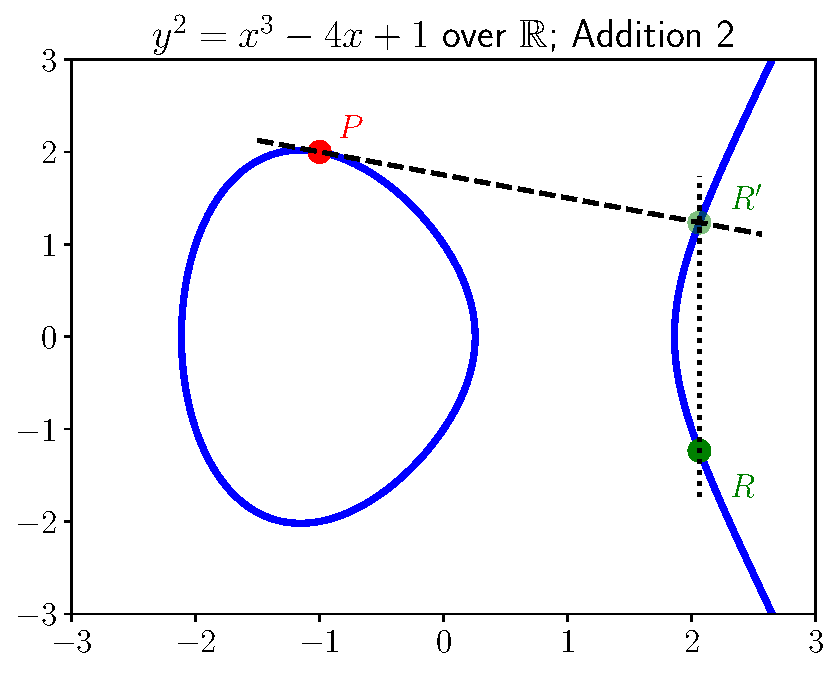
\includegraphics[width=0.70\textwidth]{plots/ec_reals/ec_reals_addition_2.pdf}
    \caption{Plot of elliptic curve addition over $\R$ for
        Example~\ref{example:ec_real_addition_2};
        this is an example of \emph{point doubling}.
        We have
        $\textcolor{red}{P} + \textcolor{red}{P} =
        \textcolor[rgb]{0,0.33,0}{R}$.
        This may also be written as
        $2\cdot\textcolor{red}{P} = \textcolor[rgb]{0,0.33,0}{R}$.
        This figure shows
        $2\cdot\textcolor{red}{\parens{-1,2}}
        = \textcolor[rgb]{0,0.33,0}{\parens{\frac{33}{16},-\frac{79}{64}}}$.}
    \label{fig:ec_real_plots_addition_2}
    \end{subfigure}

\caption[Plots of elliptic curve addition over the reals]{Here
    we plot elliptic curve addition over $\R$
    for Examples~\ref{example:ec_real_addition_1}
    and \ref{example:ec_real_addition_2}.
    Figure~\ref{fig:ec_real_plots_addition_1} shows the addition
    of distinct points while
    Figure~\ref{fig:ec_real_plots_addition_2} shows the addition
    of repeated points (point doubling).}
\label{fig:ec_real_plots_addition}
\end{figure}


\begin{example}[Elliptic Curve Addition over Reals 1]
\label{example:ec_real_addition_1}
We now look at addition on the \gls{elliptic curve}

\begin{equation}
    E: y^{2} = x^{3} - 4x + 1
\end{equation}

\noindent
over $\R$.
We want to add the two points

\begin{align}
    \textcolor{red}{P} &= \parens{0,1} \nonumber\\
    \textcolor{orange}{Q} &= \parens{2,-1}.
\end{align}

\noindent
Using the addition formula, we find

\begin{align}
    s &= -1 \nonumber\\
    x_{3} &= -1 \nonumber\\
    y_{3} &= -2.
\end{align}

\noindent
This gives us the point

\begin{equation}
    \textcolor[rgb]{0,0.33,0}{R} = \parens{-1,-2}.
\end{equation}

\noindent
Thus, we have

\begin{equation}
    \textcolor{red}{\parens{0,1}} + \textcolor{orange}{\parens{2,-1}}
    = \textcolor[rgb]{0,0.33,0}{\parens{-1,-2}}.
\end{equation}

\noindent
See Figure~\ref{fig:ec_real_plots_addition_1}
for a plot.

To understand how $\textcolor[rgb]{0,0.33,0}{R}$ is determined,
we look at the line connecting
$\textcolor{red}{P}$ and $\textcolor{orange}{Q}$.
This line will intersect the \gls{elliptic curve} at another point
$\textcolor[rgb]{0,0.33,0}{R'}$;
it can be shown that this will always happen.
The point $\textcolor[rgb]{0,0.33,0}{R}$ is defined to be
the reflection of $\textcolor[rgb]{0,0.33,0}{R'}$
across the $x$-axis.
\end{example}

\begin{example}[Elliptic Curve Addition over Reals 2]
\label{example:ec_real_addition_2}
We use the same \gls{elliptic curve} in
Example~\ref{example:ec_real_addition_1}:

\begin{equation}
    E: y^{2} = x^{3} - 4x + 1
\end{equation}

\noindent
over $\R$.

In this example, we look at adding a point to itself;
this is also called \emph{point doubling}.
In this case, we have the point

\begin{equation}
    \textcolor{red}{P} = \parens{-1,2}.
\end{equation}

\noindent
We see

\begin{align}
    s &= -\frac{1}{4} \nonumber\\
    x_{3} &= \frac{33}{16} \nonumber\\
    y_{3} &= -\frac{79}{64}.
\end{align}

\noindent
This gives us the point

\begin{equation}
    \textcolor[rgb]{0,0.33,0}{R} = \parens{\frac{33}{16},-\frac{79}{64}}.
\end{equation}

\noindent
Thus, we have

\begin{equation}
    \textcolor{red}{\parens{-1,2}} + \textcolor{red}{\parens{-1,2}}
    = \textcolor[rgb]{0,0.33,0}{\parens{\frac{33}{16},-\frac{79}{64}}}.
\end{equation}

\noindent
This may also be written as

\begin{equation}
    2\cdot\textcolor{red}{\parens{-1,2}}
    = \textcolor[rgb]{0,0.33,0}{\parens{\frac{33}{16},-\frac{79}{64}}}.
\end{equation}

\noindent
See Figure~\ref{fig:ec_real_plots_addition_2}
for a plot.

To understand how $\textcolor[rgb]{0,0.33,0}{R}$ is determined,
we now look at the tangent line of $\textcolor{red}{P}$
on the \gls{elliptic curve}.
This line will intersect the \gls{elliptic curve} at another point
$\textcolor[rgb]{0,0.33,0}{R'}$;
it can be shown that this will always happen.
The point $\textcolor[rgb]{0,0.33,0}{R}$ is defined to be
the reflection of $\textcolor[rgb]{0,0.33,0}{R'}$
across the $x$-axis.
\end{example}


\subsection{Elliptic Curves over General Fields}

We let $K$ be a \gls{field}.
For concreteness, the reader may assume $K = \R$ as before.
We are interested in looking at points $\parens{x,y}\in K^{2}$
which satisfy the equation

\begin{equation}
    E: y^{2} = x^{3} + ax + b
    \label{eq:weierstrass_form}
\end{equation}

\noindent
for $a,b\in K$.
\Glspl{elliptic curve} given in the form in Eq.~\eqref{eq:weierstrass_form}
are said to be in \emph{Weierstrass form}.
We will see other forms of \glspl{elliptic curve}
in Chapter~\ref{ssec:specific_curves}
when we discuss some specific \glspl{elliptic curve} which are used in practice.
The addition law we discussed in
Chapter~\ref{ssec:math_elliptic_addition}
is the same provided the field operations over $K$ are used.

The set of points of an \gls{elliptic curve} along with the addition
formula gives rise to an \gls{abelian group}.
We can look at cyclic subgroups of the \glspl{elliptic curve} to specify
a \gls{dlp}.

We note that there are some technical restrictions on $a$ and $b$
in Eq.~\eqref{eq:weierstrass_form},
but we do not discuss the specifics here.


\subsection{Elliptic Curves over Finite Fields}

We now focus on looking at \glspl{elliptic curve} over the
\gls{field} $\F_{p}$ for prime $p$.
Example plots can be found in Figures~\ref{fig:ec_finite_plots_1}
and \ref{fig:ec_finite_plots_2}
where we look at \glspl{elliptic curve} over $\F_{71}$.

\begin{figure}[p]
\centering
    \begin{subfigure}[t]{0.45\textwidth}
    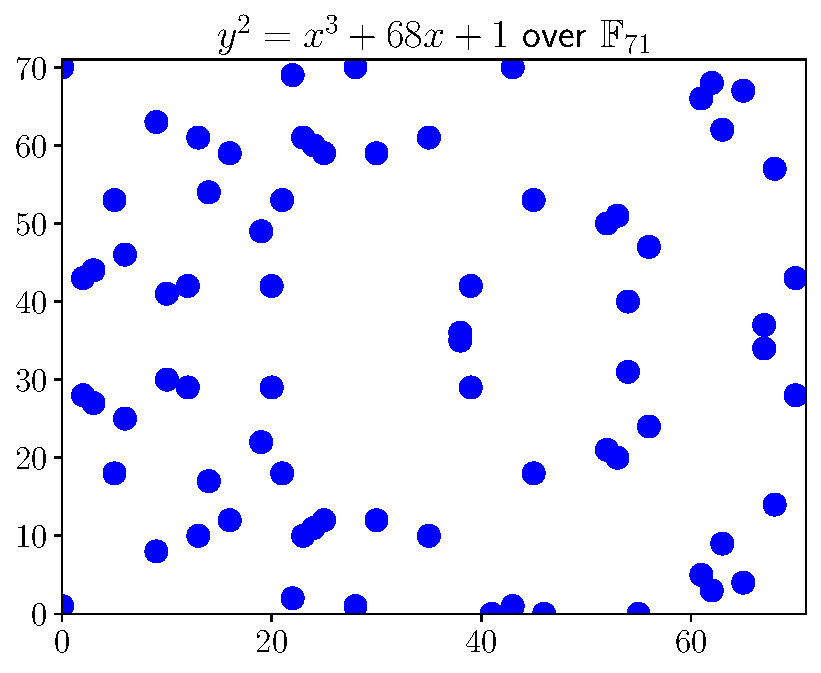
\includegraphics[width=\textwidth]{plots/ec_finite/ec_finite_F_71_68_1.pdf}
    \end{subfigure}
    \begin{subfigure}[t]{0.45\textwidth}
    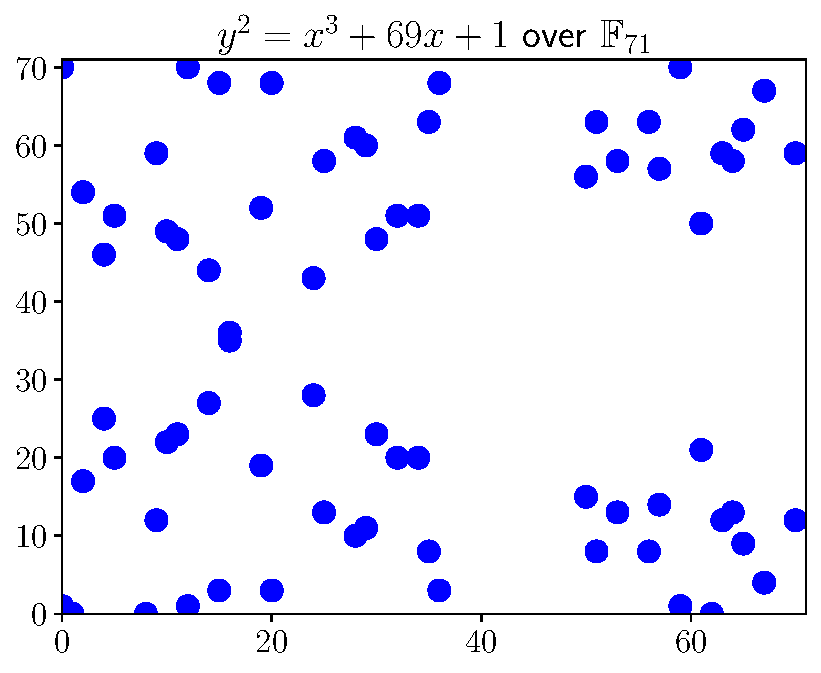
\includegraphics[width=\textwidth]{plots/ec_finite/ec_finite_F_71_69_1.pdf}
    \end{subfigure}

    \begin{subfigure}[t]{0.45\textwidth}
    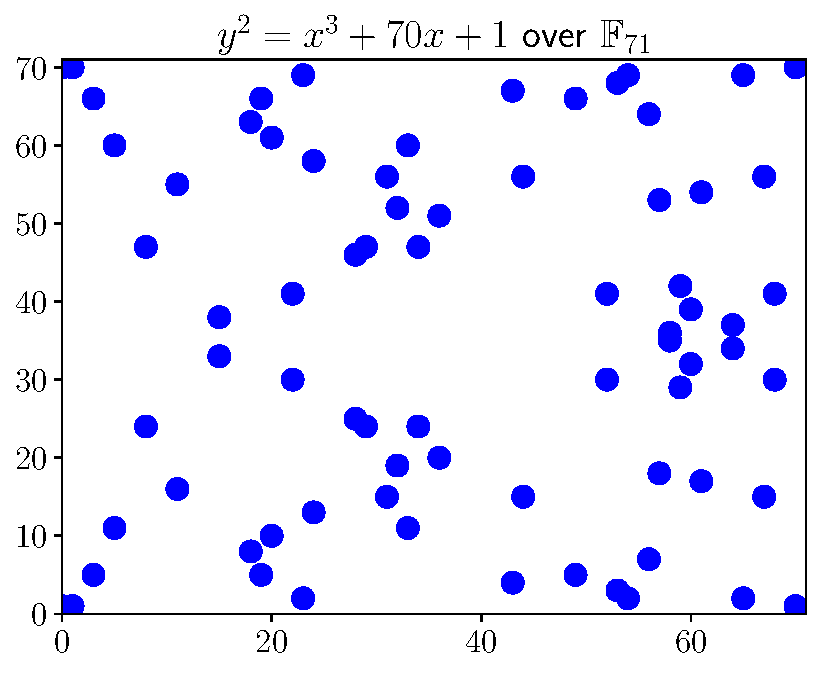
\includegraphics[width=\textwidth]{plots/ec_finite/ec_finite_F_71_70_1.pdf}
    \end{subfigure}
    \begin{subfigure}[t]{0.45\textwidth}
    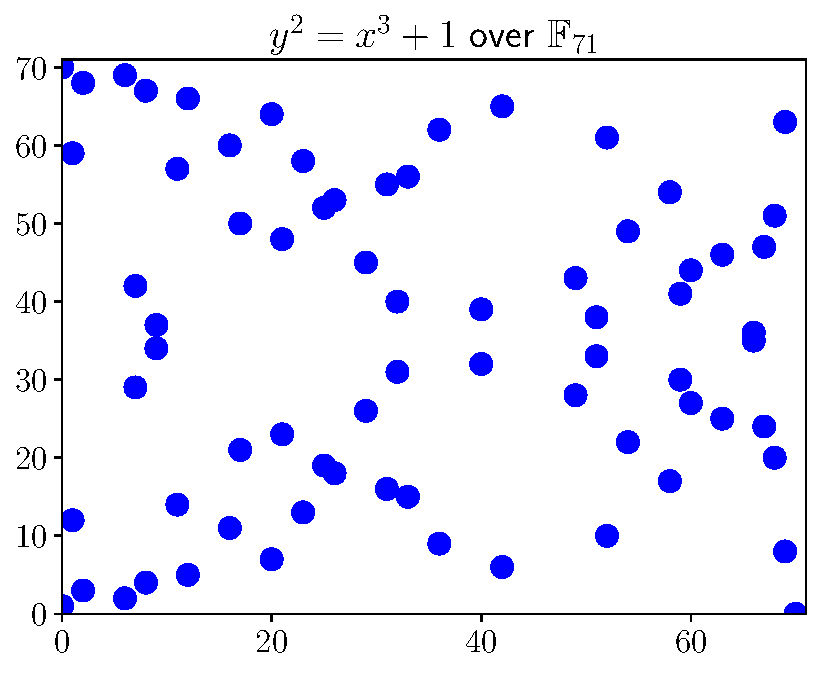
\includegraphics[width=\textwidth]{plots/ec_finite/ec_finite_F_71_0_1.pdf}
    \end{subfigure}

    \begin{subfigure}[t]{0.45\textwidth}
    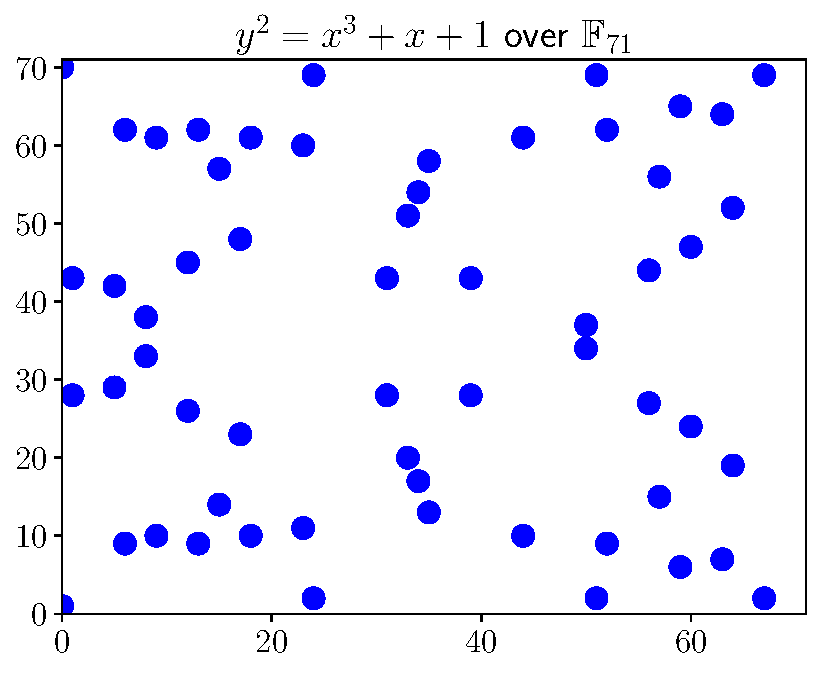
\includegraphics[width=\textwidth]{plots/ec_finite/ec_finite_F_71_1_1.pdf}
    \end{subfigure}
    \begin{subfigure}[t]{0.45\textwidth}
    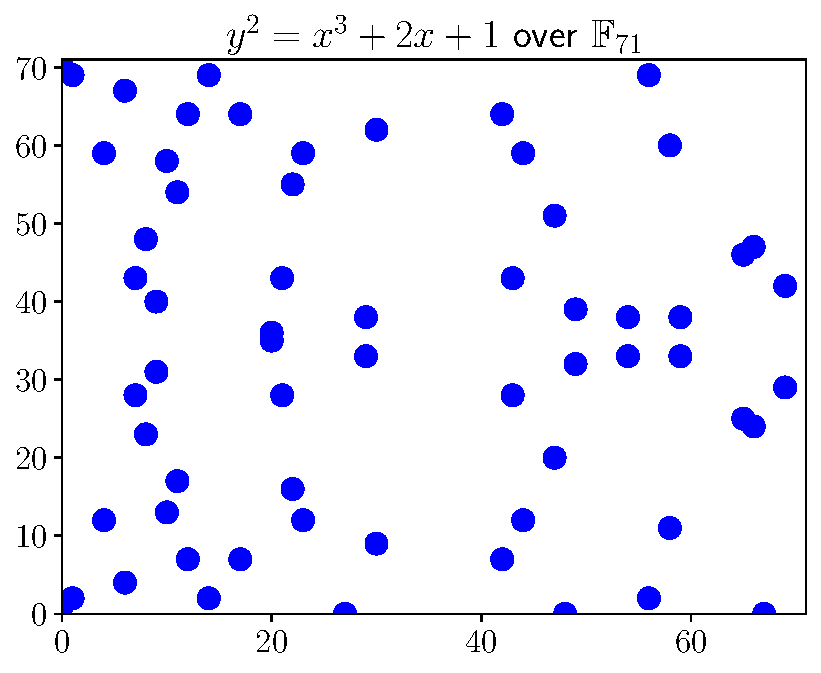
\includegraphics[width=\textwidth]{plots/ec_finite/ec_finite_F_71_2_1.pdf}
    \end{subfigure}
    \caption[Plots of elliptic curves over finite fields 1]{Here
        are plots of \glspl{elliptic curve} over $\F_{71}$.
        Here, we are keeping $b$ constant.}
    \label{fig:ec_finite_plots_1}
\end{figure}

\begin{figure}[p]
\centering
    \begin{subfigure}[t]{0.45\textwidth}
    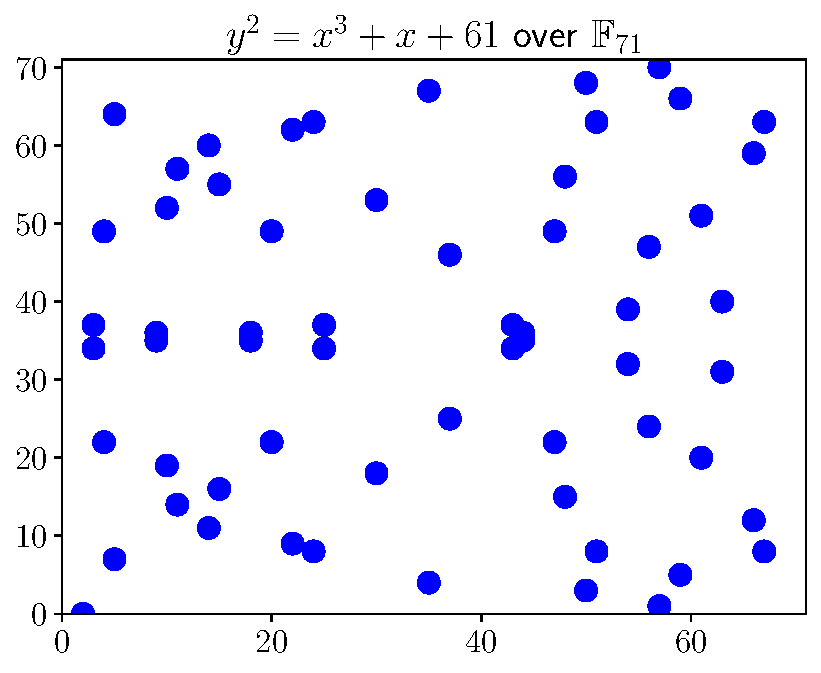
\includegraphics[width=\textwidth]{plots/ec_finite/ec_finite_F_71_1_61.pdf}
    \end{subfigure}
    \begin{subfigure}[t]{0.45\textwidth}
    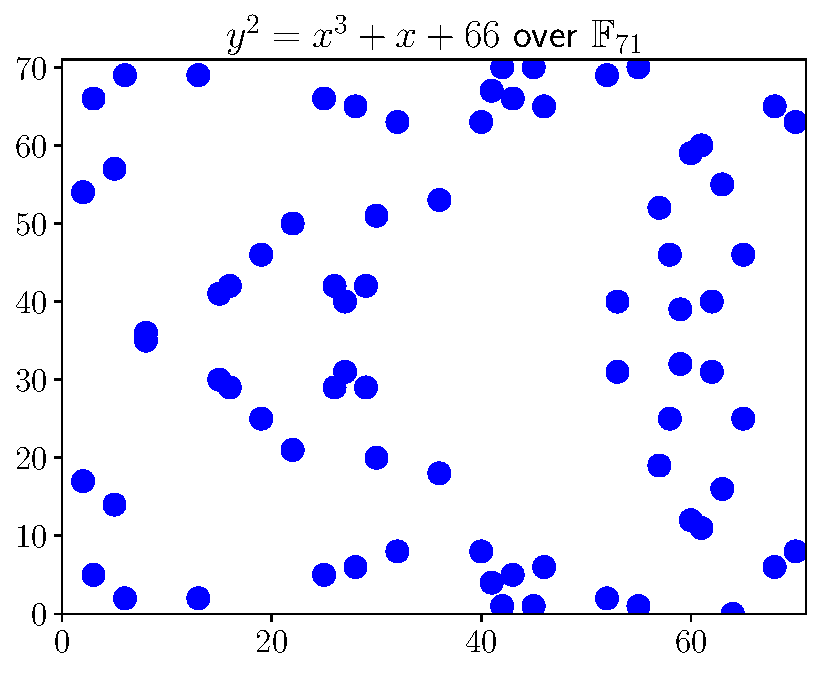
\includegraphics[width=\textwidth]{plots/ec_finite/ec_finite_F_71_1_66.pdf}
    \end{subfigure}

    \begin{subfigure}[t]{0.45\textwidth}
    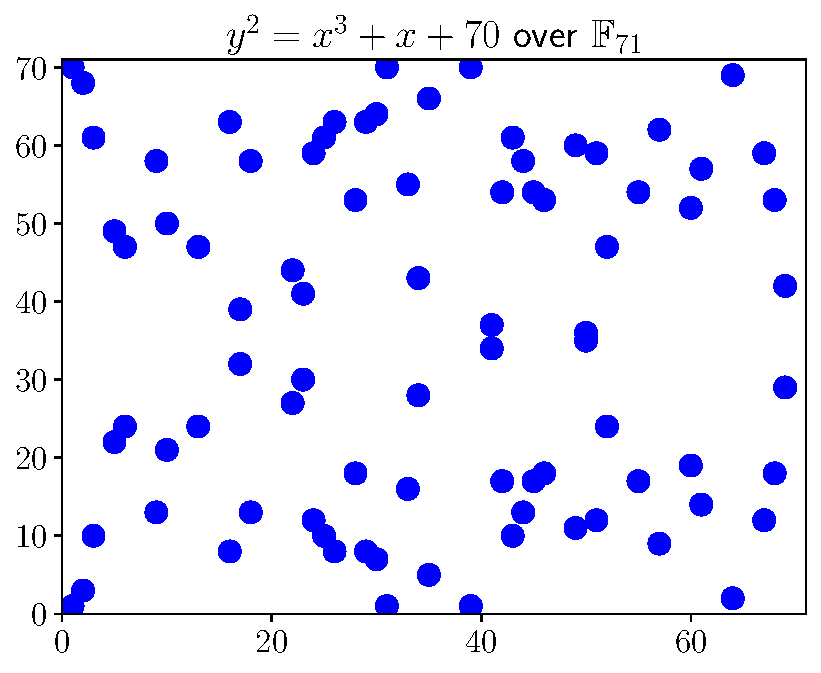
\includegraphics[width=\textwidth]{plots/ec_finite/ec_finite_F_71_1_70.pdf}
    \end{subfigure}
    \begin{subfigure}[t]{0.45\textwidth}
    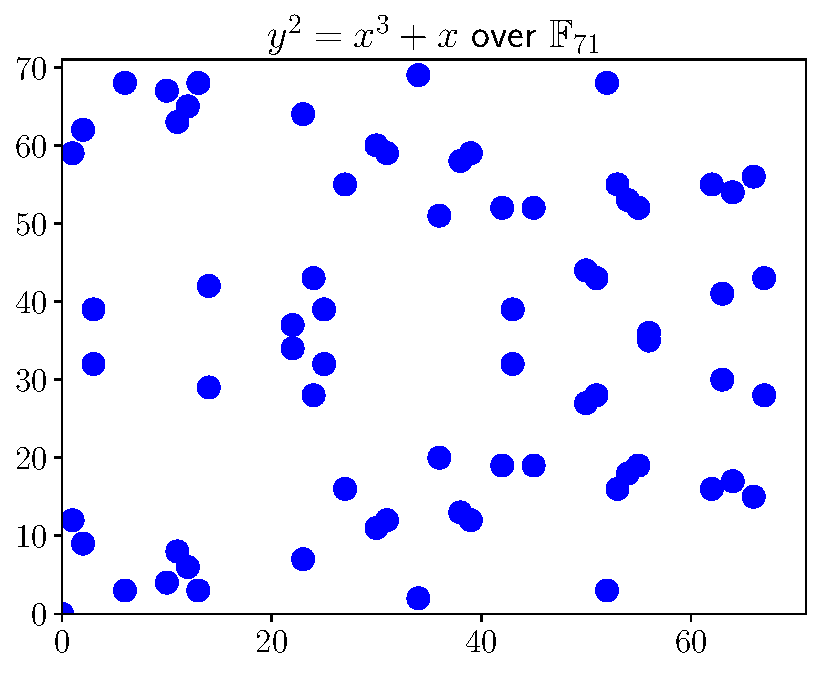
\includegraphics[width=\textwidth]{plots/ec_finite/ec_finite_F_71_1_0.pdf}
    \end{subfigure}

    \begin{subfigure}[t]{0.45\textwidth}
    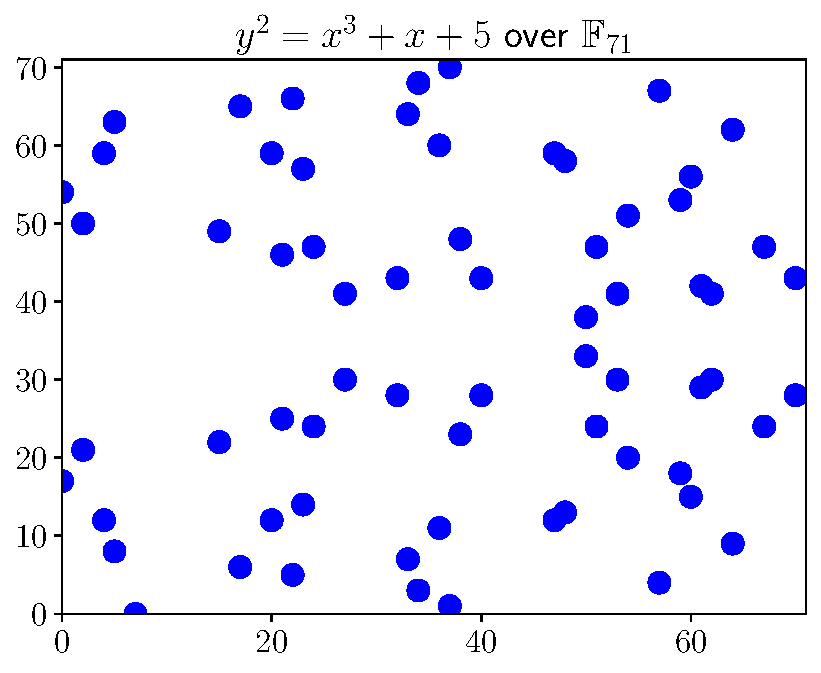
\includegraphics[width=\textwidth]{plots/ec_finite/ec_finite_F_71_1_5.pdf}
    \end{subfigure}
    \begin{subfigure}[t]{0.45\textwidth}
    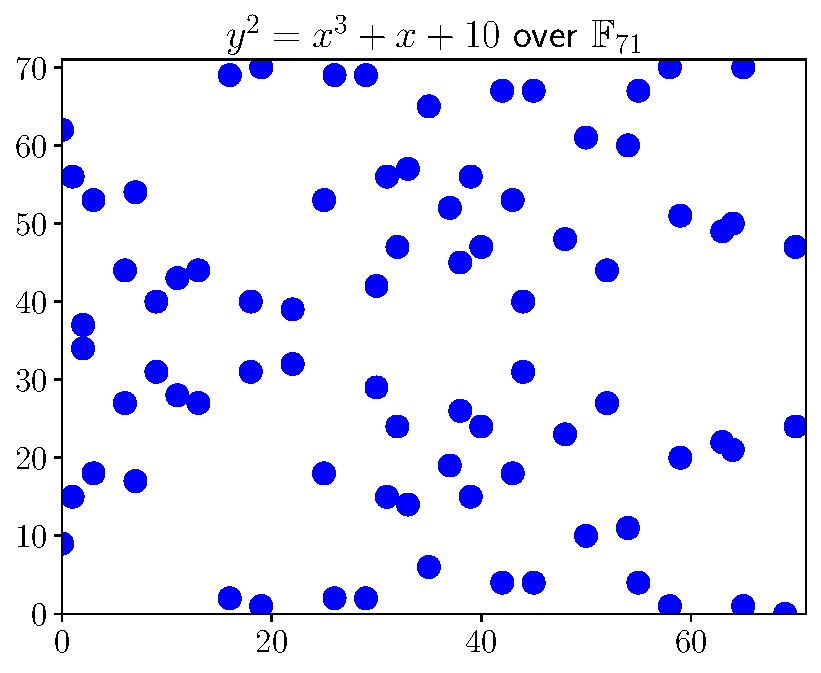
\includegraphics[width=\textwidth]{plots/ec_finite/ec_finite_F_71_1_10.pdf}
    \end{subfigure}
    \caption[Plots of elliptic curves over finite fields 2]{Here
        are additional plots of \glspl{elliptic curve} over $\F_{71}$.
        Here, we are keeping $a$ constant.}
    \label{fig:ec_finite_plots_2}
\end{figure}


The \glspl{elliptic curve} are the ``same'' as the ones in
Figures~\ref{fig:ec_real_plots_1} and \ref{fig:ec_real_plots_2}.
That is, the \emph{equation} describing each of them is the same;
the only difference is that we are now looking for solutions
over a different \gls{field}; we are looking for solutions over $\F_{71}$
rather than $\R$.
By looking at the plots, there does not appear to any relationship
between the parameters and the points on the \gls{elliptic curve}.
We still note the symmetry about the middle of the graph, though.
This comes from the $y^{2} = \cdots$ in the equation definition.

To understand the symmetry about the middle of the graph,
we will spend a bit more time discussing this.
First, we remember that, in our \glspl{finite field}, we have

\begin{equation}
    -y = p-y \mod p.
\end{equation}

\begin{figure}[p]
\centering
    \begin{subfigure}[t]{0.9\textwidth}
    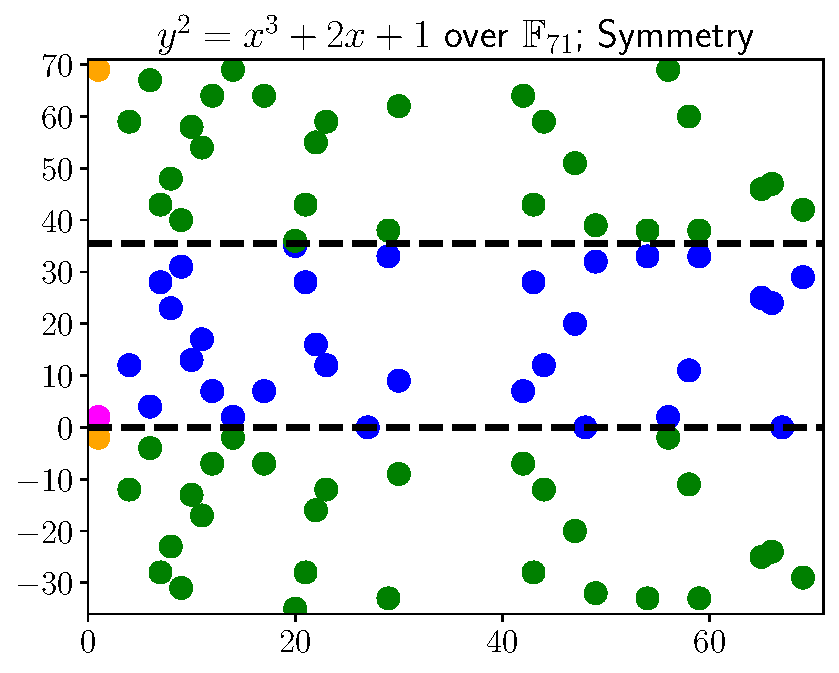
\includegraphics[width=\textwidth]{plots/ec_finite/ec_finite_F_71_2_1_symmetry_base.pdf}
    \caption{Plot with all $y$ values in $\brackets{-p/2,p}$.}
    \label{fig:ec_finite_plots_symmetry_main}
    \end{subfigure}

    \begin{subfigure}[t]{0.45\textwidth}
    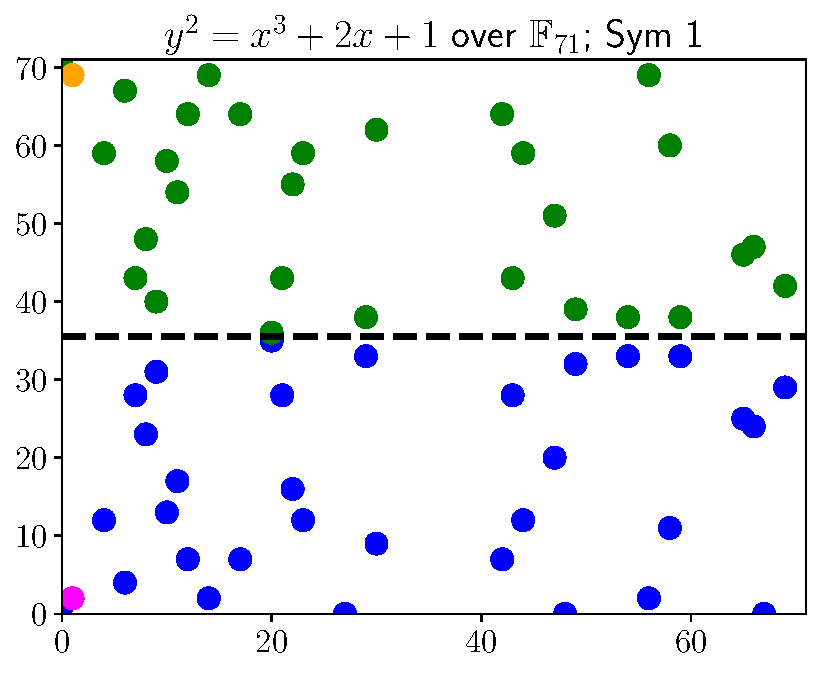
\includegraphics[width=\textwidth]{plots/ec_finite/ec_finite_F_71_2_1_symmetry_1.pdf}
    \caption{Plot with $y$ values in $\brackets{0,p}$.}
    \label{fig:ec_finite_plots_symmetry_1}
    \end{subfigure}
    \begin{subfigure}[t]{0.45\textwidth}
    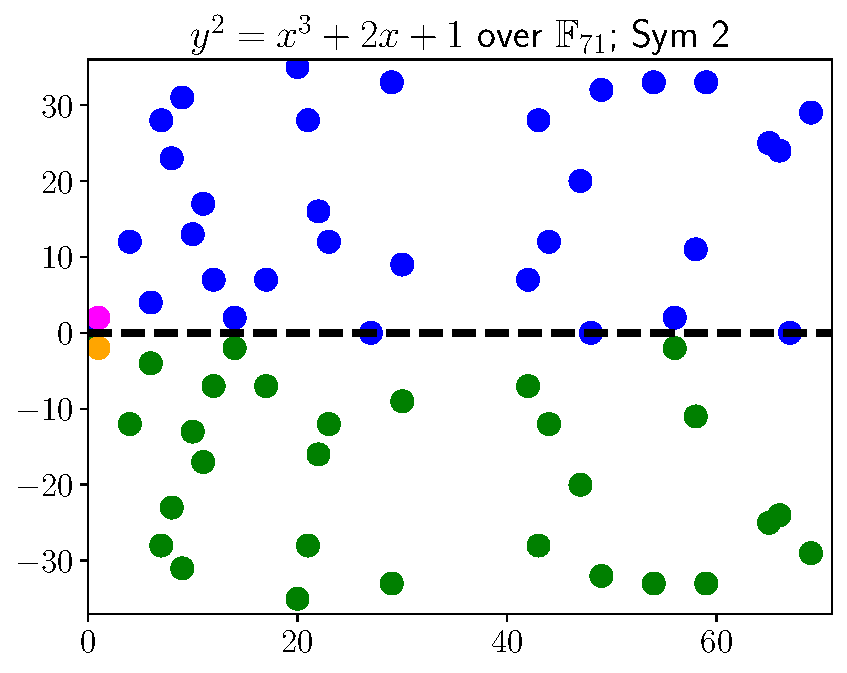
\includegraphics[width=\textwidth]{plots/ec_finite/ec_finite_F_71_2_1_symmetry_2.pdf}
    \caption{Plot with $y$ values in $\brackets{-p/2,p/2}$.}
    \label{fig:ec_finite_plots_symmetry_2}
    \end{subfigure}
\caption[Plots showing symmetry of elliptic curves over finite fields]{Here
    have a plot showing the symmetry of \glspl{elliptic curve} over $\F_{71}$.
    The ``positive'' points are in \textcolor{blue}{blue}
        with $y$-values between $0$ and $p/2$;
    the ``negative'' points are in \textcolor[rgb]{0,0.33,0}{green}
        with $y$-values between $p/2$ and $p$.
    Because $-y = p-y\mod p$,
    the negative points are equivalent to those with $y$ values
    between $-p/2$ and $0$.
    }
\label{fig:ec_finite_plots_symmetry}
\end{figure}


\noindent
To be concrete, we will focus on $y^{2} = x^{3} + 2x + 1$ over $\F_{71}$;
see Figure~\ref{fig:ec_finite_plots_symmetry_main}.
We can see \emph{two} lines of symmetry:
one line at $y=0$; another line at $y=p/2$.
These two lines of symmetry arise from $-y = p-y \mod p$:
we are free in where we put the ``negative'' numbers.
We can place the ``negative'' numbers between $p/2$ and $p$ as seen in
Figure~\ref{fig:ec_finite_plots_symmetry_1};
or we can place the ``negative'' numbers between $-p/2$ and $0$ as seen in
Figure~\ref{fig:ec_finite_plots_symmetry_2}.
In all of our plots, we will use the first convention
and always have plot $y$ values between $0$ and $p$.
Within Figure~\ref{fig:ec_finite_plots_symmetry},
we have a distinguished point $\color{magenta}{\parens{1,2}}$.
The additive inverse of this point is
$\color{orange}{\parens{1,-2}}$.
This is equivalent to $\color{orange}{\parens{1,69}}$
over $\F_{71}$.

All of the previous plots looked at \glspl{elliptic curve} over $\F_{71}$.
Even so, the particular form of \gls{elliptic curve} depends on the
\gls{finite field} as well.
Figure~\ref{fig:ec_finite_plots_fields} includes some plots where
we keep the equation fixed but change the prime $p$.

\begin{figure}[p]
\centering
    \begin{subfigure}[t]{0.45\textwidth}
    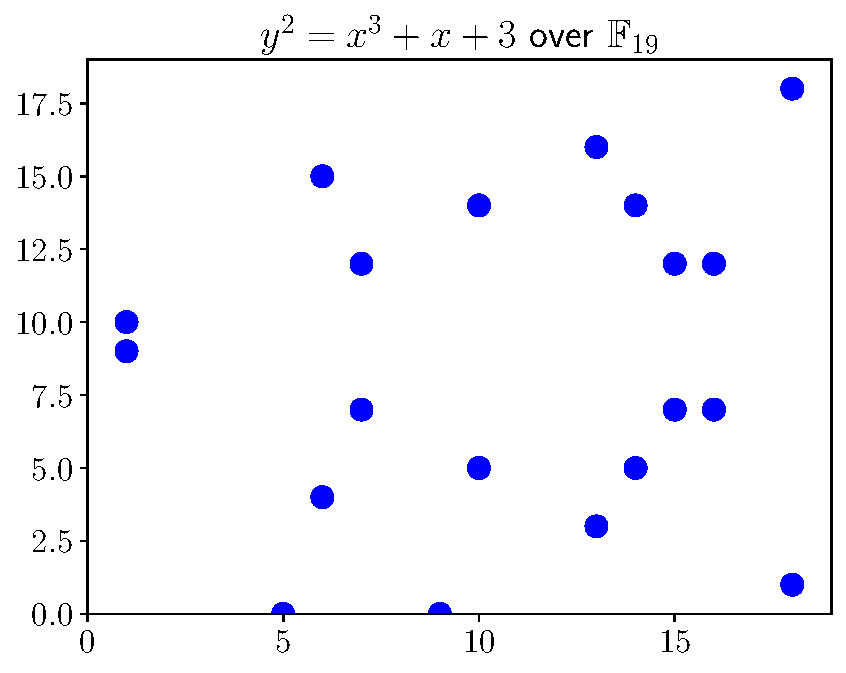
\includegraphics[width=\textwidth]{plots/ec_finite/ec_finite_F_19_1_3.pdf}
    \end{subfigure}
    \begin{subfigure}[t]{0.45\textwidth}
    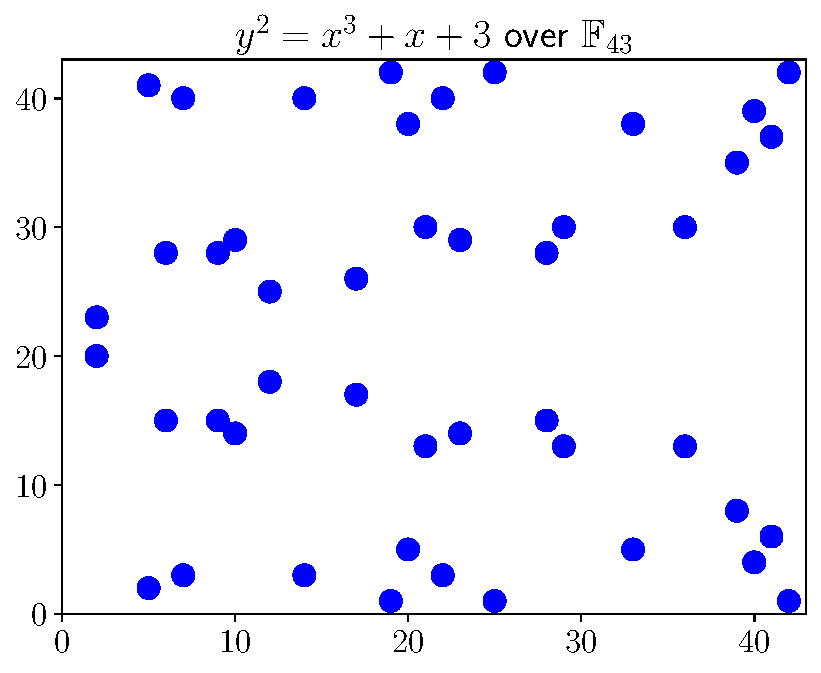
\includegraphics[width=\textwidth]{plots/ec_finite/ec_finite_F_43_1_3.pdf}
    \end{subfigure}

    \begin{subfigure}[t]{0.45\textwidth}
    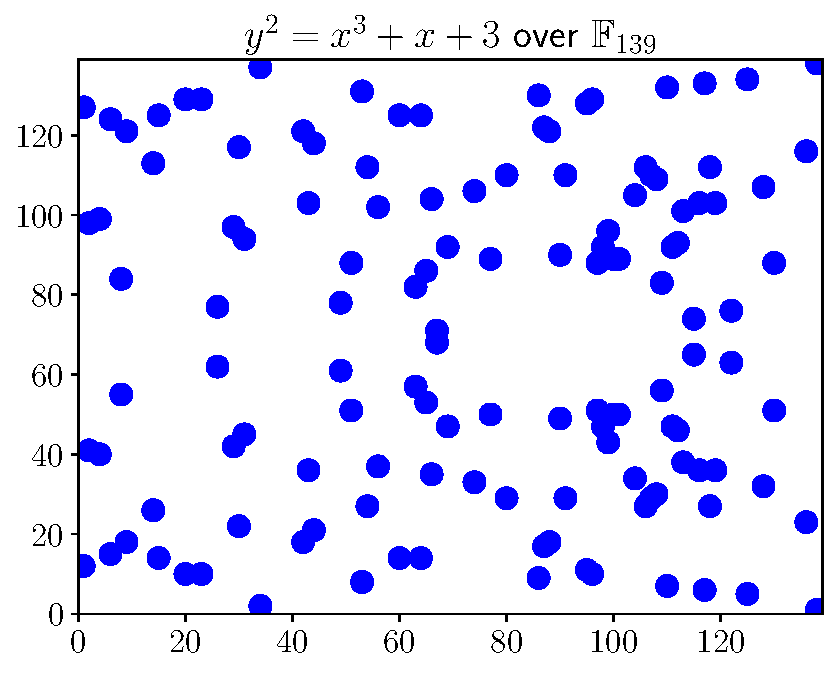
\includegraphics[width=\textwidth]{plots/ec_finite/ec_finite_F_139_1_3.pdf}
    \end{subfigure}
    \begin{subfigure}[t]{0.45\textwidth}
    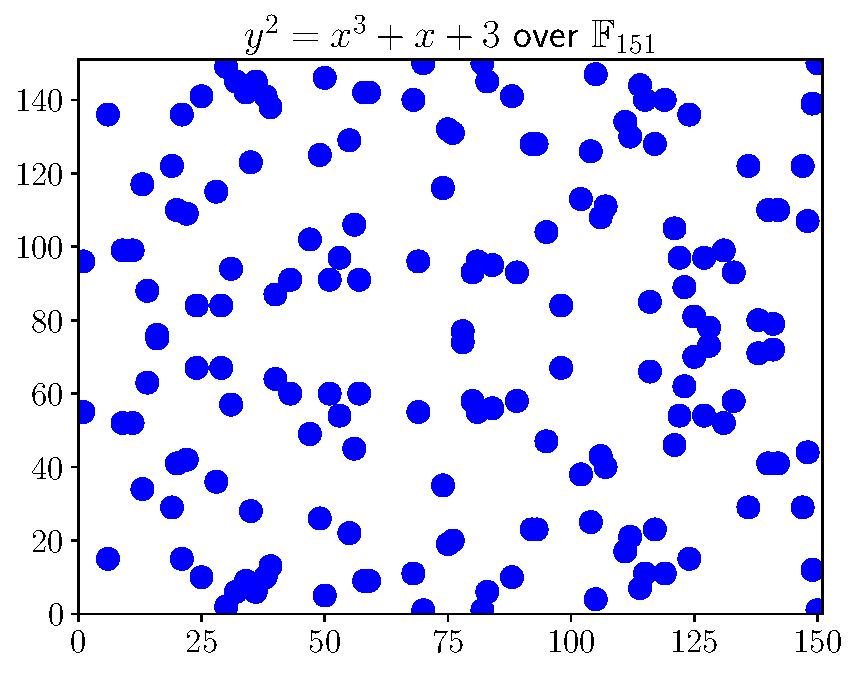
\includegraphics[width=\textwidth]{plots/ec_finite/ec_finite_F_151_1_3.pdf}
    \end{subfigure}

    \begin{subfigure}[t]{0.45\textwidth}
    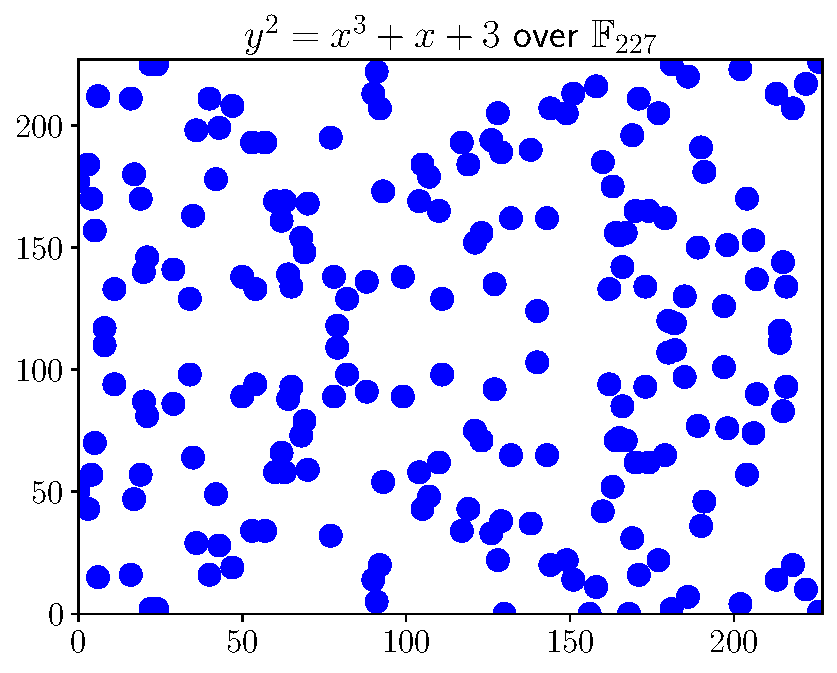
\includegraphics[width=\textwidth]{plots/ec_finite/ec_finite_F_227_1_3.pdf}
    \end{subfigure}
    \begin{subfigure}[t]{0.45\textwidth}
    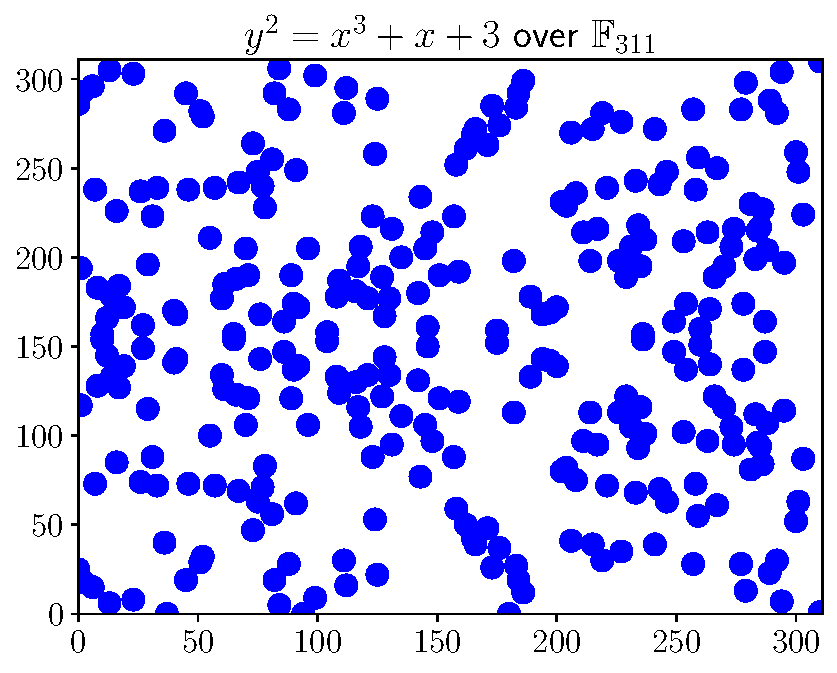
\includegraphics[width=\textwidth]{plots/ec_finite/ec_finite_F_311_1_3.pdf}
    \end{subfigure}
    \caption[Plots of elliptic curves over various finite fields]{Here
        are plots of \glspl{elliptic curve} over $\F_{p}$
        for primes $p\in\braces{19, 43, 139, 151, 227, 311}$.}
    \label{fig:ec_finite_plots_fields}
\end{figure}


We have not talked about methods to determine how many points
are on a specific \gls{elliptic curve}.
There are methods to compute the exact number of
elements on an \gls{elliptic curve},
but we will not discuss them here.
Here is an easy bound on the number of points:

\begin{thm}[{{Hasse's Theorem on Elliptic Curves~\cite[Theorem V.1.1]{AEC}}}]
\label{thm:hasse_bound}
Let $\#E(\F_{p})$ denote the number of elements of an \gls{elliptic curve}
$E/\F_{p}$.
Then we have the following bound:

\begin{equation}
    \abs{\#E(\F_{p}) - \parens{p+1}} \le 2\sqrt{p}.
\end{equation}
\end{thm}

\noindent
This means that the number of points on the \gls{elliptic curve}
$E\parens{\F_{p}}$ is essentially $p$.

We now look at some examples of addition on \glspl{elliptic curve}.
By looking at the points and the \gls{elliptic curve},
there does not appear to be any structure.

\begin{example}[Addition of Elliptic Curves over Finite Fields]
\exampleCodeReference{examples/math\_review/elliptic\_curve\_addition.py}

We will focus on the \gls{elliptic curve}

\begin{equation}
    E: y^{2} = x^{3} + 2x + 1
\end{equation}

\noindent
over $\F_{71}$.

We compute the following values:

\begin{align}
    \parens{17,7} + \parens{20,35} &= \parens{58,60}
        \nonumber\\
    \parens{17,7} + \parens{21,28} &= \parens{65,25}
        \nonumber\\
    \parens{17,7} + \parens{22,16} &= \parens{4,59}
        \nonumber\\
    \parens{17,7} + \parens{23,12} &= \parens{10,58}
        \nonumber\\
    \parens{17,7} + \parens{29,33} &= \parens{8,48}.
\end{align}

\noindent
We plot the results of addition in Figure~\ref{fig:ec_finite_plots_addition}.

\begin{figure}[p]
\centering
    \begin{subfigure}[t]{0.45\textwidth}
    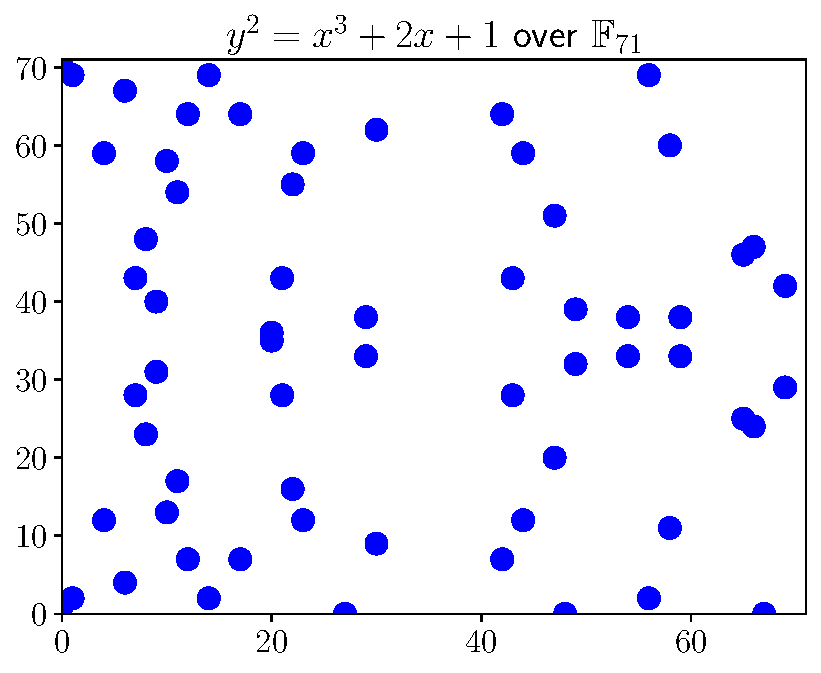
\includegraphics[width=\textwidth]{plots/ec_finite/ec_finite_F_71_2_1_addition_base.pdf}
    \caption{All points on $y^{2} = x^{3} + 2x + 1$ over $\F_{71}$.}
    \end{subfigure}
    \begin{subfigure}[t]{0.45\textwidth}
    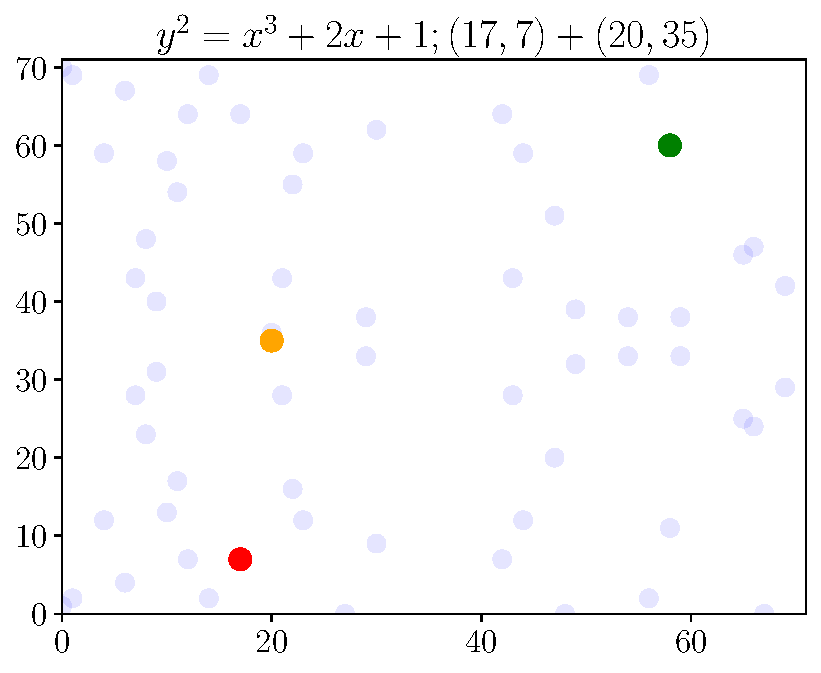
\includegraphics[width=\textwidth]{plots/ec_finite/ec_finite_F_71_2_1_addition_20_35.pdf}
    \caption{$\textcolor{red}{\parens{17,7}}
        + \textcolor{orange}{\parens{20,35}}
        = \textcolor[rgb]{0,0.33,0}{\parens{58,60}}$}
    \end{subfigure}

    \begin{subfigure}[t]{0.45\textwidth}
    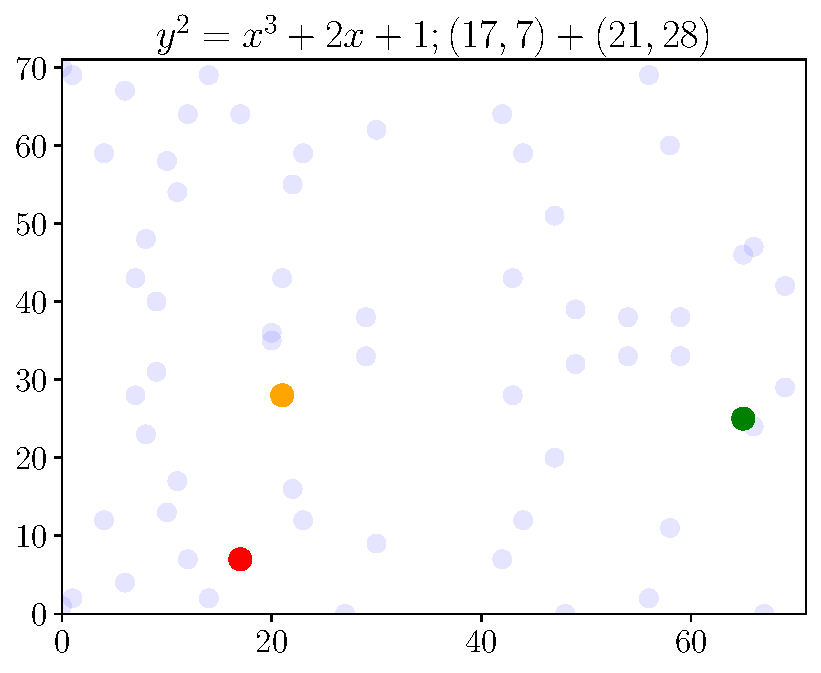
\includegraphics[width=\textwidth]{plots/ec_finite/ec_finite_F_71_2_1_addition_21_28.pdf}
    \caption{$\textcolor{red}{\parens{17,7}}
        + \textcolor{orange}{\parens{21,28}}
        = \textcolor[rgb]{0,0.33,0}{\parens{65,25}}$}
    \end{subfigure}
    \begin{subfigure}[t]{0.45\textwidth}
    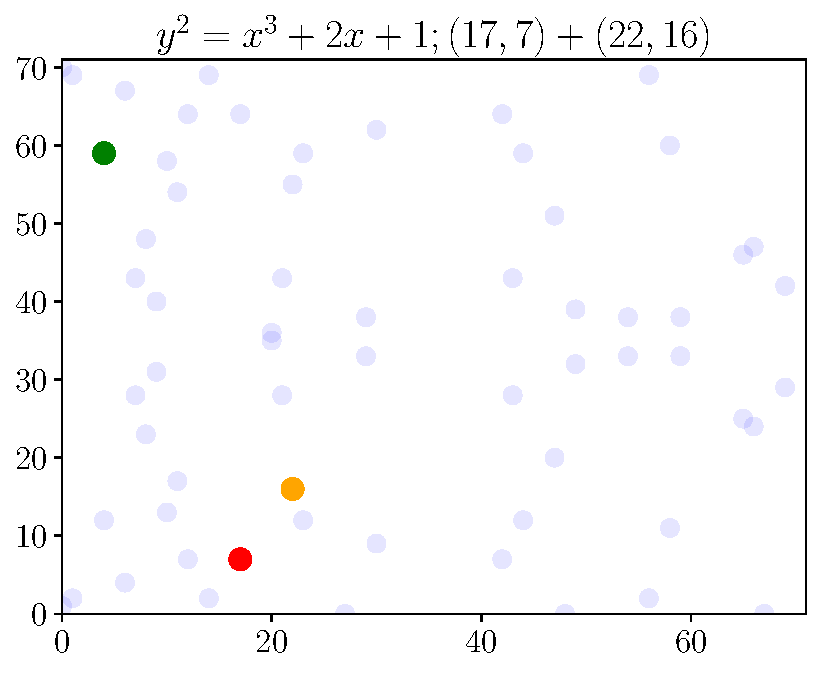
\includegraphics[width=\textwidth]{plots/ec_finite/ec_finite_F_71_2_1_addition_22_16.pdf}
    \caption{$\textcolor{red}{\parens{17,7}}
        + \textcolor{orange}{\parens{22,16}}
        = \textcolor[rgb]{0,0.33,0}{\parens{4,59}}$}
    \end{subfigure}

    \begin{subfigure}[t]{0.45\textwidth}
    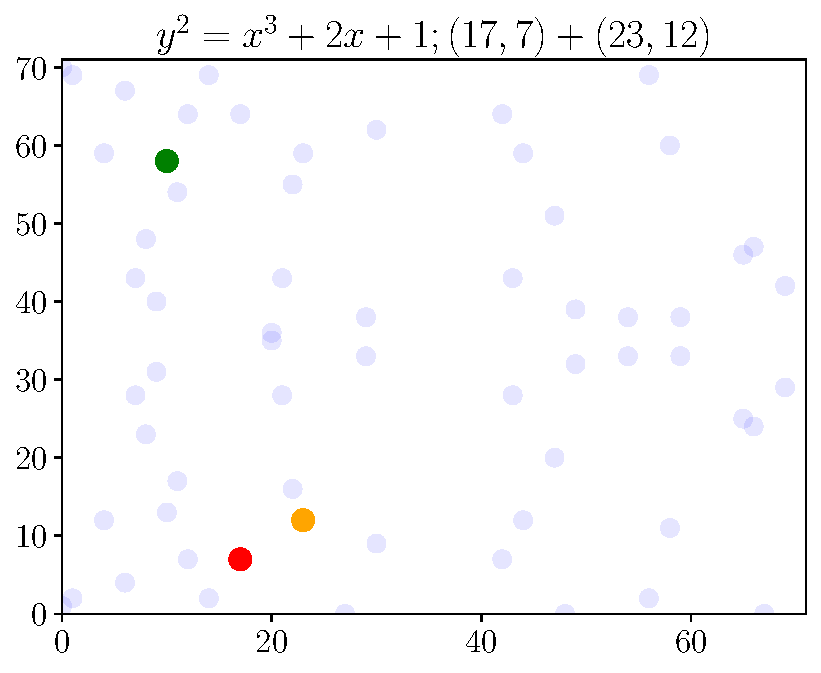
\includegraphics[width=\textwidth]{plots/ec_finite/ec_finite_F_71_2_1_addition_23_12.pdf}
    \caption{$\textcolor{red}{\parens{17,7}}
        + \textcolor{orange}{\parens{23,12}}
        = \textcolor[rgb]{0,0.33,0}{\parens{10,58}}$}
    \end{subfigure}
    \begin{subfigure}[t]{0.45\textwidth}
    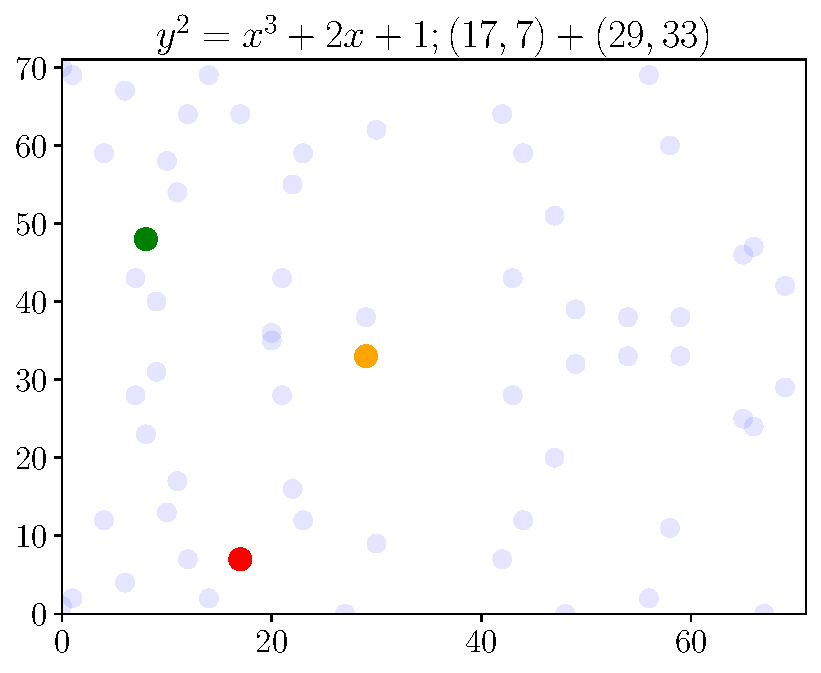
\includegraphics[width=\textwidth]{plots/ec_finite/ec_finite_F_71_2_1_addition_29_33.pdf}
    \caption{$\textcolor{red}{\parens{17,7}}
        + \textcolor{orange}{\parens{29,33}}
        = \textcolor[rgb]{0,0.33,0}{\parens{8,48}}$}
    \end{subfigure}
    \caption[Plots of elliptic curve addition over finite fields]{Here
        have plots of addition on \glspl{elliptic curve} over $\F_{71}$.
        The \glspl{elliptic curve} are all the same: $y^{2} = x^{3} + 2x + 1$.
        The first plot shows the points on the \gls{elliptic curve};
        the other plots show the addition
        $\textcolor{red}{P} + \textcolor{orange}{Q}
            = \textcolor[rgb]{0,0.33,0}{R}$.
        Throughout the plots, $\color{red} P = \parens{17,7}$.
        }
    \label{fig:ec_finite_plots_addition}
\end{figure}

\end{example}


\subsection{Elliptic Curve Scalar Multiplication}
\label{ssec:ec_scalar_mult}

In Chapter~\ref{ssec:ec_subgroups}, we will want to repeatedly add
a point on an \gls{elliptic curve} to itself.
That is, we will want to compute $k\cdot P$ for $k\in\Z$
and $P\in E\parens{\F_{p}}$.
This is defined as

\begin{equation}
    k\cdot P \mathDef{} 
        \underbrace{P + P + \cdots + P}_{\text{$k$ times}}, \quad k\ge 0.
\end{equation}

\noindent
Similarly, we have

\begin{equation}
    k\cdot P \mathDef{} 
        \underbrace{-P - P - \cdots - P}_{\text{$-k$ times}}, \quad k< 0.
\end{equation}

\noindent
This is called \emph{elliptic curve point multiplication} or
\emph{elliptic curve scalar multiplication}.
We remember that if $P\in E(\F_{p})$ and $E$ is in Weierstrass form
with $P = \parens{x,y}$, then $-P = \parens{x,-y}$.
Thus, point negation has negligible cost.

We recall that, in practice, we will define \glspl{elliptic curve} over
$\F_{p}$ with $p$ being a 256-bit prime number.
Thus, $k$ will also be a 256-bit number.
Computing $k\cdot P$ by performing

\begin{align}
    2P &= P + P  \nonumber\\
    3P &= P + 2P \nonumber\\
    4P &= P + 3P \nonumber\\
    5P &= P + 4P \nonumber\\
    &\vdots
\end{align}

\noindent
would take around $2^{256}$ elliptic curve additions.
There is not a fast enough computer to perform the calculation
using this method.

Thankfully, there is a better method called the \emph{double-and-add} method;
see Alg.~\ref{alg:ec_double_and_add} for a formal specification
using \gls{recursion}.
We will walk through the method in Example~\ref{example:ec_double-and-add}.

\begin{algorithm}[t]
\caption{Double-and-add formula for elliptic curve
    scalar multiplication}
\label{alg:ec_double_and_add}
\begin{algorithmic}[1]
\Require $P$ point on \gls{elliptic curve}; $k\in\N$
\Procedure{DoubleAndAdd}{$P$, $k$}
    \If {$k=0$}
        \State \Return $\mathcal{O}$
    \ElsIf {$k=1$}
        \State \Return $P$
    \ElsIf {$k\equiv0\mod 2$}
        \State \Return $\textsc{DoubleAndAdd}(P+P, k/2)$
    \Else
        \State \Return $\textsc{DoubleAndAdd}(P+P, (k-1)/2)+P$
    \EndIf
\EndProcedure
\end{algorithmic}
\end{algorithm}


While this is an efficient algorithm to compute $k\cdot P$,
the branch logic will \emph{leak information} about $k$.
For instance, this type of operation occurs when $k$
could be a private key.
Thus, if this operation is not performed in a secure method
\emph{independent} of $k$, the private key could be
revealed~\cite{cryptoeprint:2014:140}.

We note that the double-and-add formula may be used
when computing large exponentiations as well;
the algorithms are the same except for switching the operations
from doubling and addition to squaring and multiplication.

\begin{example}[Double-and-Add Example]
\label{example:ec_double-and-add}
\exampleCodeReference{examples/math\_review/elliptic\_curve\_double-and-add.py}

We continue using the \gls{elliptic curve}

\begin{equation}
    E: y^{2} = x^{3} + 2x + 1
\end{equation}

\noindent
defined over $\F_{71}$ as before.
We want to compute

\begin{equation}
    29\cdot\parens{0,1}.
\end{equation}

We will use Alg.~\ref{alg:ec_double_and_add}.
We first see that

\begin{equation}
    \parens{0,1} + \parens{0,1} = \parens{1,69}.
\end{equation}

\noindent
We have

\begin{equation}
    \textsc{DoubleAndAdd}\brackets{\parens{0,1}, 29}
    = \parens{0,1} + \textsc{DoubleAndAdd}\brackets{\parens{1,69}, 14}.
\end{equation}

\noindent
Next, we see

\begin{equation}
    \parens{1,69} + \parens{1,69} = \parens{4,59}.
\end{equation}

\noindent
We then compute

\begin{equation}
    \textsc{DoubleAndAdd}\brackets{\parens{1,69}, 14}
    = \textsc{DoubleAndAdd}\brackets{\parens{4,59}, 7}.
\end{equation}

\noindent
In the next step, we find

\begin{equation}
    \parens{4,59} + \parens{4,59} = \parens{56,2}.
\end{equation}

\noindent
After this, we have

\begin{equation}
    \textsc{DoubleAndAdd}\brackets{\parens{4,59}, 7}
    = \parens{4,59} + \textsc{DoubleAndAdd}\brackets{\parens{56,2}, 3}.
\end{equation}

\noindent
Another addition gives us

\begin{equation}
    \parens{56,2} + \parens{56,2} = \parens{67,0}.
\end{equation}

\noindent
The final iteration gives us

\begin{align}
    \textsc{DoubleAndAdd}\brackets{\parens{56,2}, 3}
        &= \parens{56,2} + \textsc{DoubleAndAdd}\brackets{\parens{67,0}, 1}
            \nonumber\\
    &= \parens{56,2} + \parens{67,0}.
\end{align}

\noindent
Our algorithm has stopped.

At this point, we can add all of the points we have computed.
Doing this, we see

\begin{align}
    29\cdot\parens{0,1} &=
            \parens{0,1} + \braces{\parens{4,59} + \brackets{
                \parens{56,2} + \parens{67,0}}}
        \nonumber\\
    &= \parens{0,1} + \braces{\parens{4,59} + \parens{56,69}}
        \nonumber\\
    &= \parens{0,1} + \parens{4,12}
        \nonumber\\
    &= \parens{8,48}.
\end{align}

\noindent
This took us 7 additions on the \gls{elliptic curve};
this is much less than 29.
\end{example}

In fact, using Alg.~\ref{alg:ec_double_and_add},
the computation is logarithmic in $k$;
that is, it will take $O(\log(k)^{c})$ steps for small constant $c>0$.


\subsection{Subgroups of Elliptic Curves over Finite Fields}
\label{ssec:ec_subgroups}

We now have the addition formula
and the ability to efficiently add points.
\emph{This} allows us to create \glspl{subgroup} of \glspl{elliptic curve}
over \glspl{finite field} for \gls{ecc}.

We let $P\in E(\F_{p})$ be a point on an \gls{elliptic curve}.
We define the following \gls{subgroup}:

\begin{equation}
    \angles{P} \mathDef{} \braces{k\cdot P \mid k\in\Z}.
\end{equation}

\noindent
Naturally, we have $\angles{P}\le E(\F_{p})$;
more explicitly, $\angles{P}$ is the \gls{subgroup}
of the \gls{elliptic curve} $E(\F_{p})$
formed by looking at all the points on the \gls{elliptic curve}
which we can get by adding $P$ to itself.
We can always look at \glspl{subgroup} of this form over general
\glspl{elliptic curve};
when we restrict our attention to \glspl{finite field},
then the \glspl{elliptic curve} are \glspl{finite group}.
These \glspl{finite group} allow us to look at the
\emph{\gls{dlp}}:
If $Q \in \angles{P}$, determine $x\in\Z$ such that

\begin{equation}
    Q = x\cdot P.
\end{equation}

\noindent
For many \glspl{elliptic curve}, this is difficult problem.
This is discussed more in Chapter~\ref{chap:hardness}.

See Figure~\ref{fig:ec_finite_plots_subgroups}
for example cyclic subgroups of \glspl{elliptic curve} over
\glspl{finite field}.

\begin{figure}[p]
\centering
    \begin{subfigure}[t]{0.45\textwidth}
    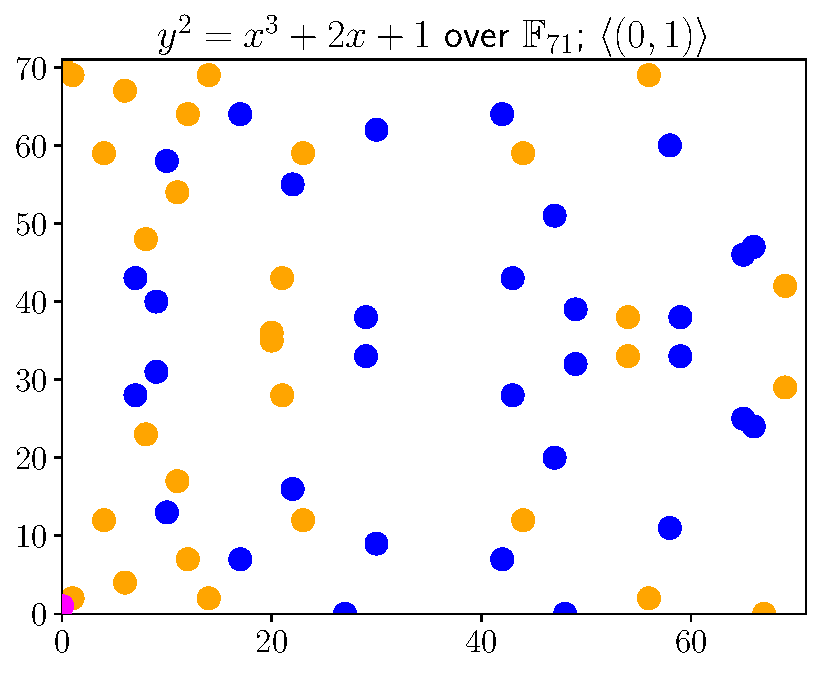
\includegraphics[width=\textwidth]{plots/ec_finite/ec_finite_F_71_2_1_subgroup_0_1.pdf}
    \caption{\textcolor{orange}{Subgroup} generated by
        $\color{magenta} \parens{0,1}$}
    \label{fig:ec_finite_plots_subgroups_0_1}
    \end{subfigure}
    \begin{subfigure}[t]{0.45\textwidth}
    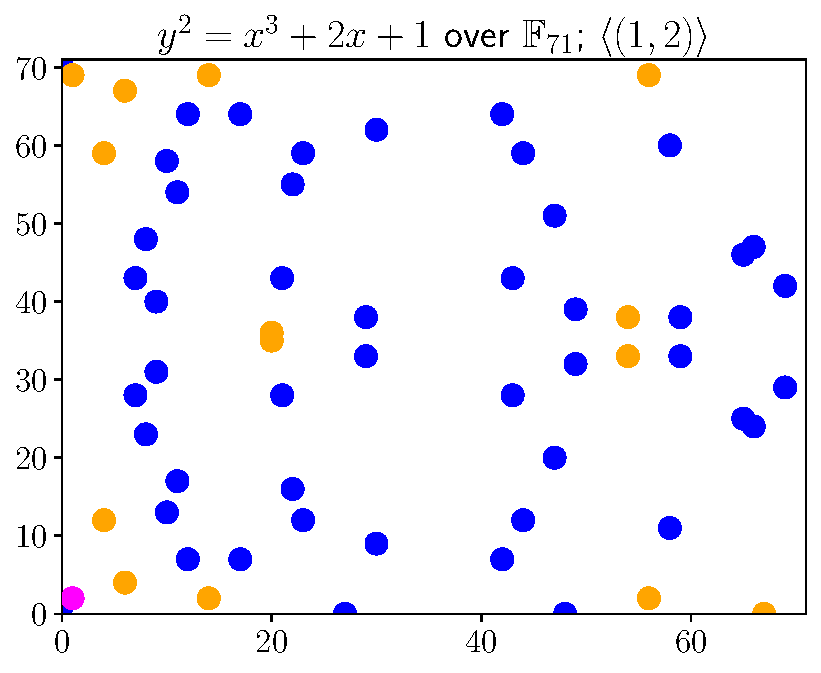
\includegraphics[width=\textwidth]{plots/ec_finite/ec_finite_F_71_2_1_subgroup_1_2.pdf}
    \caption{\textcolor{orange}{Subgroup} generated by
        $\color{magenta}\parens{1,2}$}
    \label{fig:ec_finite_plots_subgroups_1_2}
    \end{subfigure}

    \begin{subfigure}[t]{0.45\textwidth}
    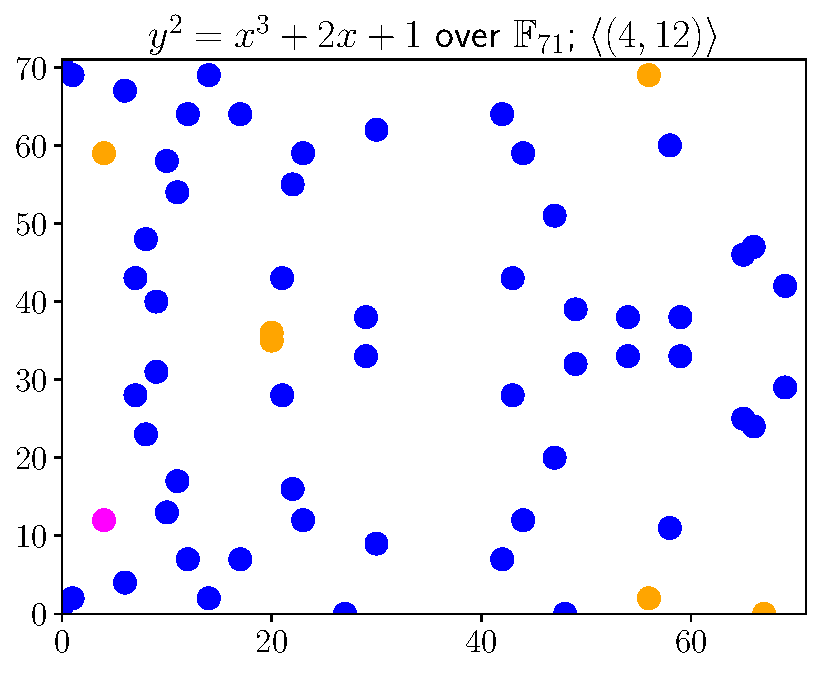
\includegraphics[width=\textwidth]{plots/ec_finite/ec_finite_F_71_2_1_subgroup_4_12.pdf}
    \caption{\textcolor{orange}{Subgroup} generated by
        $\color{magenta}\parens{4,12}$}
    \label{fig:ec_finite_plots_subgroups_4_12}
    \end{subfigure}
    \begin{subfigure}[t]{0.45\textwidth}
    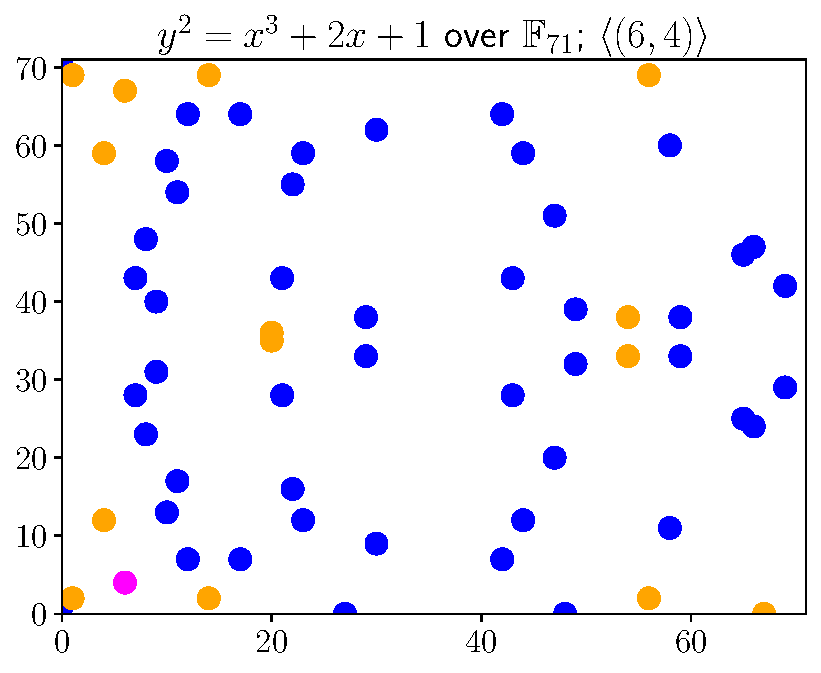
\includegraphics[width=\textwidth]{plots/ec_finite/ec_finite_F_71_2_1_subgroup_6_4.pdf}
    \caption{\textcolor{orange}{Subgroup} generated by
        $\color{magenta}\parens{6,4}$}
    \label{fig:ec_finite_plots_subgroups_6_4}
    \end{subfigure}

    \begin{subfigure}[t]{0.45\textwidth}
    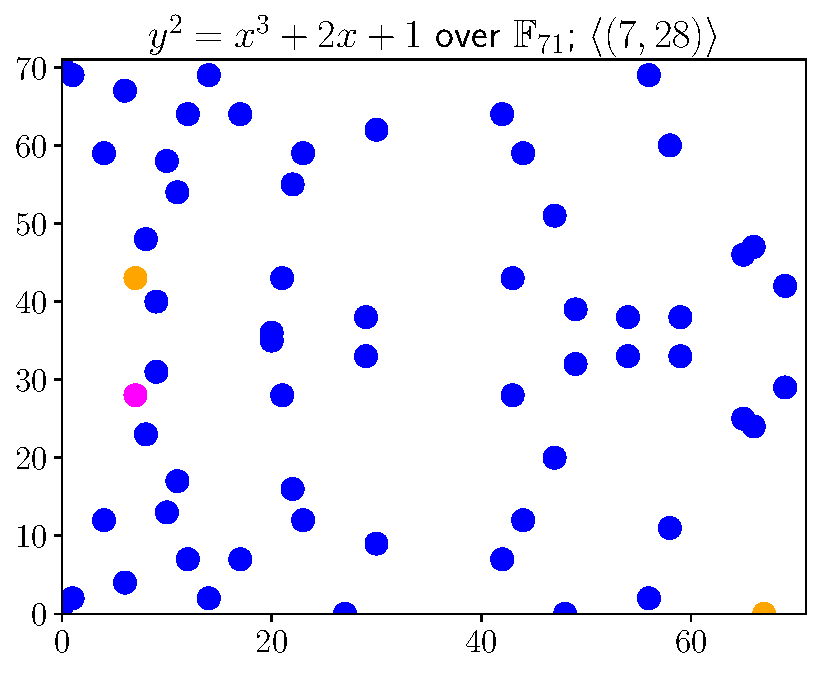
\includegraphics[width=\textwidth]{plots/ec_finite/ec_finite_F_71_2_1_subgroup_7_28.pdf}
    \caption{\textcolor{orange}{Subgroup} generated by
        $\color{magenta}\parens{7,28}$}
    \label{fig:ec_finite_plots_subgroups_7_28}
    \end{subfigure}
    \begin{subfigure}[t]{0.45\textwidth}
    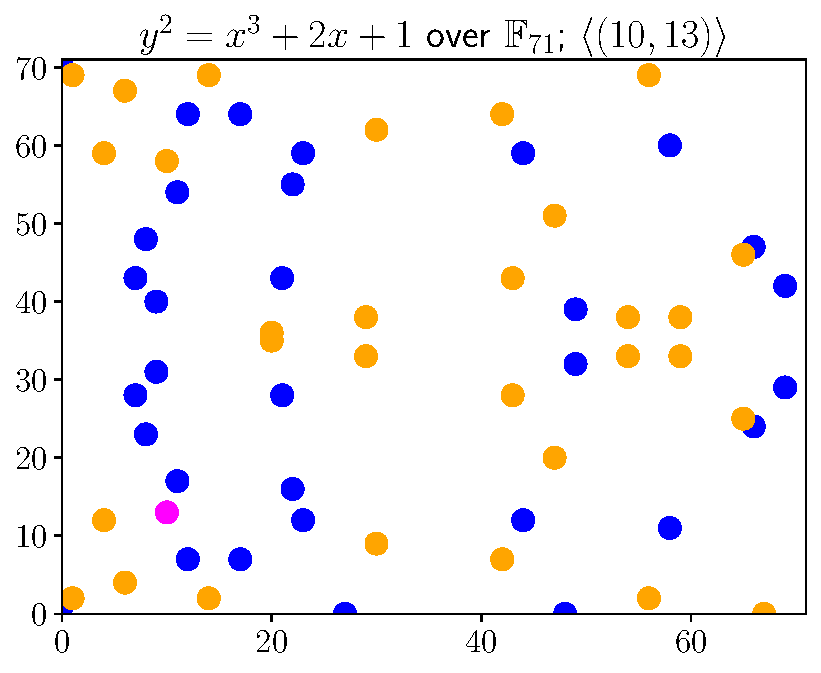
\includegraphics[width=\textwidth]{plots/ec_finite/ec_finite_F_71_2_1_subgroup_10_13.pdf}
    \caption{\textcolor{orange}{Subgroup} generated by
        $\color{magenta}\parens{10,13}$}
    \label{fig:ec_finite_plots_subgroups_10_13}
    \end{subfigure}
    \caption[Plots of subgroups of elliptic curves over finite fields]{Here
        are plots of \glspl{elliptic curve} over $\F_{71}$.
        The \glspl{elliptic curve} are all the same: $y^{2} = x^{3} + 2x + 1$.
        In each plot, we also show different cyclic subgroups;
        \textcolor{orange}{subgroups} generated by different
        \textcolor{magenta}{base points}.}
    \label{fig:ec_finite_plots_subgroups}
\end{figure}


\begin{example}[Subgroups of Elliptic Curves]
\exampleCodeReference{examples/math\_review/elliptic\_curve\_subgroup.py}

In this example we look at \glspl{subgroup} on an \gls{elliptic curve}.
We will focus on the \gls{elliptic curve}

\begin{equation}
    E: y^{2} = x^{3} + 2x + 1
\end{equation}

\noindent
over $\F_{71}$.
Plots of various \glspl{subgroup} are found in
Figure~\ref{fig:ec_finite_plots_subgroups}.

We will focus on $\angles{\parens{1,2}}$;
this can be seen in
Figure~\ref{fig:ec_finite_plots_subgroups_1_2}.
If we list out all the points of the \gls{subgroup}, we see

\begin{align}
    1\cdot \parens{1,2}  &= \parens{1,2}
        &
    9\cdot \parens{1,2}  &= \parens{6,67} \nonumber\\
    2\cdot \parens{1,2}  &= \parens{4,12}
        &
    10\cdot \parens{1,2} &= \parens{20,35} \nonumber\\
    3\cdot \parens{1,2}  &= \parens{14,2}
        &
    11\cdot \parens{1,2} &= \parens{54,33} \nonumber\\
    4\cdot \parens{1,2}  &= \parens{56,69}
        &
    12\cdot \parens{1,2} &= \parens{56,2} \nonumber\\
    5\cdot \parens{1,2}  &= \parens{54,38}
        &
    13\cdot \parens{1,2} &= \parens{14,69} \nonumber\\
    6\cdot \parens{1,2}  &= \parens{20,36}
        &
    14\cdot \parens{1,2} &= \parens{4,59} \nonumber\\
    7\cdot \parens{1,2}  &= \parens{6,4}
        &
    15\cdot \parens{1,2} &= \parens{1,69} \nonumber\\
    8\cdot \parens{1,2}  &= \parens{67,0}
        &
    16\cdot \parens{1,2} &= \mathcal{O}.
    \label{eq:elliptic_ecdlp}
\end{align}

\noindent
As we look at the point distribution and compare it with
the rest of the points,
there does not appear to be any structure between
the points in the \gls{subgroup} or not.
It is this apparent lack of structure that makes \gls{elliptic curve}
\glspl{group} great for \gls{publiccrypto}.

We note that the \glspl{subgroup} in
Figures~\ref{fig:ec_finite_plots_subgroups_1_2}
and \ref{fig:ec_finite_plots_subgroups_6_4} are the same;
this means that the points $\parens{1,2}$ and $\parens{6,4}$
generate the same \glspl{subgroup}.
\end{example}

\begin{example}[Elliptic Curve Discrete Logarithm]
We continue the previous example with the same \gls{elliptic curve}
and \gls{subgroup}.

We want to find $x$ such that

\begin{equation}
    x\cdot\parens{1,2} = \parens{54,33}.
\end{equation}

\noindent
Because the addition formula for points on \glspl{elliptic curve} is ``random'',
there does not appear to be any better way to find
$x$ than to just list out every possibility.
From looking at all the scalar multiplications
in Eq.~\eqref{eq:elliptic_ecdlp},
we see that $x = 11$.
\end{example}

We note that generic methods for solving the \gls{elliptic curve} \gls{dlp}
are discussed in Chapter~\ref{sec:hardness_dlp}.


\subsection{Elliptic Curve Point Compression}
\label{ssec:ec_point_compression}

Due to the fact that \glspl{elliptic curve} satisfy an algebraic equation,
we are able to \emph{compress} points on the \gls{elliptic curve}
so that they take up less space.

We assume that $p$ is an odd prime.
As before, let us look at an \gls{elliptic curve} $E/\F_{p}$
and suppose that we have a point on the \gls{elliptic curve}
$P = \parens{x,y}$.
We know that we have the relation

\begin{equation}
    y^{2} = x^{3} + ax + b.
\end{equation}

\noindent
for some specified $a,b\in\F_{p}$.

If we only knew $x$, then we can solve for $y$:

\begin{equation}
    y = \pm\sqrt{x^{3} + ax + b}.
\end{equation}

\noindent
The challenge is to then determine \emph{which} $y$ value
is the appropriate one.
We see that such a square root must exist, so we set

\begin{equation}
    s \mathDef{} \sqrt{x^{3} + ax + b}.
    \label{eq:ec_compress_sqrt}
\end{equation}

\noindent
Note well that this square root is a \emph{modular square root},
not a regular square root.
Thus, we have

\begin{equation}
    y = \pm s.
\end{equation}

Now, we remember that all of these operations are modular arithmetic
operations modulo a prime $p$.
Thus, we know $s\in\braces{0, 1, 2, \cdots, p-1}$.
We also remember that

\begin{equation}
    -s = p - s \mod p.
\end{equation}

\noindent
Because we are assuming that $p$ is an odd prime,
we know there are two possibilities:
$s$ is even and $p-s$ is odd; or
$s$ is odd and $p-s$ is even.

We can use these facts to compress the point $P = \parens{x,y}$
on an \gls{elliptic curve};
this allows for more efficient transmission.
For instance, suppose that $p$ is an $n$-bit prime.
In this case, the uncompressed form of representing $P$
requires $2n$ bits.
The compressed form only requires $n+1$ bits: $n$ bits to store $x$
and $1$ bit to store whether $y$ is even or odd.
By using the compressed form, storage is essentially halved.
This assumes that the particular \gls{elliptic curve} being used
is public knowledge so that $a$ and $b$ are known.

We did not mention \emph{how} to compute $s$ in
Eq.~\eqref{eq:ec_compress_sqrt}.
Methods for computing square roots in \glspl{finite field}
may be found in Appendix~\ref{app:math_finite_fields}.

\begin{example}[Elliptic Curve Point Compression]
\exampleCodeReference{examples/math\_review/elliptic\_curve\_compression.py}

We continue to work with the \gls{elliptic curve}

\begin{equation}
    E: y^{2} = x^{3} + 2x + 1
\end{equation}

\noindent
over $\F_{71}$.

If we want to compress the point $\parens{17,7}$,
then we need to send $\parens{17,\texttt{0b1}}$;
we send \texttt{0b1} because the $y$-coordinate $7$ is odd.

Suppose we receive the compressed point $\parens{47,\texttt{0b0}}$.
Thus, the $x$-coordinate is $47$ and the $y$-coordinate is even.
We see that

\begin{align}
    t &\mathDef{} x^{3} + ax + b \mod p\nonumber\\
        &= 47^{3} + 2\cdot47 + 1 \mod 71 \nonumber\\
        &= 45.
\end{align}

\noindent
We can verify that

\begin{equation}
    51^{2} \mod 71 = 45.
\end{equation}

\noindent
Thus, $51$ is a square root of $45$.
It follows that

\begin{align}
    s &\mathDef{} \sqrt{t} \mod p \nonumber\\
        &= 51.
\end{align}

\noindent
We note, though, that $s$ is odd although we were told $y$ is even;
thus, we have

\begin{align}
    y &\mathDef{} p - s \nonumber\\
        &= 20.
\end{align}

\noindent
Therefore, the point in uncompressed form is

\begin{equation}
    P = \parens{47,20}.
\end{equation}
\end{example}

As we can see from the above example,
the point compression for \glspl{elliptic curve} trades
storage for computation.
Compression may be worthwhile in situations where
storage is relatively expensive.

\subsection{Examples of Specific Curves}
\label{ssec:specific_curves}

We now include some specific curves used in practice.
We also bring them up because some of them have forms different
than the Weierstrass form we have been using.

While it is very easy to come up with additional \glspl{elliptic curve},
developing new \glspl{elliptic curve} for cryptography requires
\emph{extreme care}.
Doing this is \emph{highly discouraged}, as it amounts to
``rolling your own crypto''.
This was frowned upon in Chapter~\ref{chap:do_not}.

Whenever possible, use a well-tested library developed by
experienced cryptologists.
If this is not possible, \emph{proceed with caution}.

\subsubsection{Secp256k1}

This \gls{elliptic curve} is used by both Bitcoin~\cite{BitcoinWhitepaper} and
\gls{ethereum}~\cite[Appendix F]{EthereumYellowpaper}
for \glspl{signature}.
It has the form

\begin{equation}
    E:y^{2} = x^{3} + 7
\end{equation}

\noindent
over the \gls{field} $\F_{q}$ with

\begin{equation}
    q = 2^{256} - 2^{32} - 2^{9} - 2^{8} - 2^{7} - 2^{6} - 2^{4} - 1.
\end{equation}

\noindent
It was defined in~\cite[Section 2.4.1]{brown2010sec2}.

\subsubsection{Curve25519}

This curve~\cite{Curve25519} is used in X25519,
the \gls{dhke} based on this curve.
We have

\begin{equation}
    E:y^{2} = x^{3} + 486662x^{2} + x
\end{equation}

\noindent
over the prime \gls{field} $\F_{q}$,
where

\begin{equation}
    q = 2^{255} - 19.
\end{equation}

\noindent
This is a \emph{Montgomery curve}.
A general Montgomery curve has the form

\begin{equation}
    M_{A,B}: By^{2} = x^{3} + Ax^{2} + x
\end{equation}

\noindent
over a field $K$ with $A,B\in K$.
Having this specific form allows for some operations to be
efficiently computed.

\subsubsection{Ed25519}

This is one of the \glspl{elliptic curve} used for the
Edwards Curve Digital Signature Algorithm (EdDSA)~\cite{ed25519}.
It is birationally equivalent to Curve25519~\cite{Curve25519}.
We have

\begin{equation}
    E:-x^{2} + y^{2} = 1 - \frac{121665}{121666}x^{2}y^{2}
\end{equation}

\noindent
over the \gls{field} $\F_{q}$ with

\begin{equation}
    q = 2^{255}-19.
\end{equation}

\noindent
This is a \emph{twisted Edwards curve}.
In general, a twisted Edwards curve has the form

\begin{equation}
    E_{E,a,d}:ax^{2} + y^{2} = 1 + dx^{2}y^{2}
\end{equation}

\noindent
over a field $K$ with $a,d\in K$ distinct.
There is a minor technical restriction on the field $K$
which we do not mention.

\subsection{Encoding Elliptic Curves over Finite Fields}

When working with the \glspl{elliptic curve} $E/\F_{p}$,
we can encode $\parens{x,y}$ using its binary representation;
encoding the identity element $\mathcal{O}$ may require care.
It may be useful to use point compression described
in Chapter~\ref{ssec:ec_point_compression} depending on the situation.

\section{Bilinear Pairings}
\label{sec:math_pairings}

\subsection{Why do we care about Bilinear Pairings?}

We care about \glspl{bilinear} because they give us a lot of nice
mathematical features that we can use.
In particular, \glspl{bilinear} give us
\emph{short digital signatures}.
These started with BLS signatures based on the Weil
pairing~\cite{BLSSignatures},
a particular type of \gls{bilinear}.

\Glspl{bilinear} also allow for threshold group signatures.
These can be formed as part of a \gls{distributed key generation}
protocol and are discussed in Chapter~\ref{chap:secret_sharing}.

\subsection{Formal Definition}

A \gls{bilinear} is a special type of \gls{function}:

\begin{defn}[Bilinear Pairing]
We let $G_{1}$, $G_{2}$, and $G_{T}$ be \glspl{finite group} with
$\abs{G_{1}} = \abs{G_{2}} = \abs{G_{T}}$.
We say $e:G_{1}\times G_{2}\to G_{T}$ is a \emph{\gls{bilinear}}
if for all $h_{1}\in G_{1}$, $h_{2}\in G_{2}$, and $a,b\in\Z$
we have

\begin{equation}
    e\parens{h_{1}^{a},h_{2}^{b}} = \brackets{e\parens{h_{1},h_{2}}}^{ab}.
\end{equation}
\end{defn}

\subsection{Discussion}

It is straightforward to \emph{use} the previous definition.
The challenge is \emph{finding} \glspl{group} with which to build such a
\gls{bilinear}.
This is nontrivial.

At this point, all \glspl{bilinear} arise from \glspl{elliptic curve}.
The exact construction is complex and we do not discuss it here.
We will use \glspl{bilinear} in Chapter~\ref{chap:pairing}
when we discuss \gls{pairingcrypto}.
Having a solid understanding of the mathematics behind pairings
and how they are constructed from \glspl{elliptic curve}
requires advanced knowledge of \glspl{elliptic curve} as discussed
in~\cite{AEC}.

\section{Lagrange Interpolation}
\label{sec:math_lagrange}

We spend some time discussing \gls{lagrange interpolation}.

\subsection{Why do we care about interpolation?}

Within cryptography, \emph{\gls{lagrange interpolation}}
over \glspl{finite field}
is used in secret sharing protocols and \gls{distributed key generation}.
More generally, interpolation is useful because
it attempts to approximate a complex function with a simpler polynomial.

We will start by looking at interpolation over real data.
After working through examples, we will transition
to interpolation over \glspl{finite field} as this is our primary focus.

\subsection{Lagrange Interpolation over the Reals}

Given a set of data points $\braces{\parens{x_{k},y_{k}}}_{k=1}^{n}$
with $\braces{x_{k}}_{k=1}^{n}$ distinct,
we want to find the interpolating polynomial of minimal degree
which agrees with the data.
That is, we want a polynomial $p$ of at most degree $n-1$ such that

\begin{equation}
    p(x_{k}) = y_{k}, \quad k\in\braces{1,\cdots,n}.
\end{equation}

We now proceed to construct such a polynomial.
To do this, we set

\begin{align}
    L(x) &\mathDef{} \sum_{k=1}^{n} y_{k}\ell_{k}(x) \nonumber\\
    \ell_{k}(x) &\mathDef{}
        \prod_{\substack{1\le j \le n \\ j\ne k}} \frac{x-x_{j}}{x_{k}-x_{j}}
            \nonumber\\
        &=
        \frac{x-x_{1}}{x_{k}-x_{1}}\cdot
        \frac{x-x_{2}}{x_{k}-x_{2}}\cdots
        \frac{x-x_{k-1}}{x_{k}-x_{k-1}}\cdot
        \frac{x-x_{k+1}}{x_{k}-x_{k+1}}\cdots
        \frac{x-x_{n}}{x_{k}-x_{n}}.
    \label{eq:math_lagrange_def}
\end{align}

\noindent
We note that $\ell_{k}$ is a polynomial of degree $n-1$;
this implies that $L$ is a polynomial of degree at most $n-1$.
We note that

\begin{align}
    \ell_{k}(x_{j}) &=
        \begin{cases} 1, \quad k = j \\ 0, \quad k\ne j \end{cases}
            \nonumber\\
        &= \del_{kj}.
\end{align}

\noindent
Here, $\del_{kj}$ is the Kronecker delta.
It follows that 

\begin{align}
    L(x_{j}) &= \sum_{k=1}^{n}y_{k}\ell_{k}(x_{j}) \nonumber\\
        &= \sum_{k=1}^{n} y_{k}\del_{kj} \nonumber\\
        &= y_{j}.
\end{align}

\noindent
Thus, this is the interpolating polynomial which agrees
with the data.
Furthermore, the degree of the polynomial is at most $n-1$.
Such polynomials are unique.

\subsection{Examples of Lagrange Interpolation over the Reals}

\begin{example}
\label{example:math_lagrange_reals_1}
\exampleCodeReference{examples/math\_review/lagrange\_reals\_1.py}

We begin by interpolating the data
$\braces{\parens{1,2},\parens{4,1},\parens{7,8}}$.
See the data in Figure~\ref{fig:lagrange_points_1}.

\begin{figure}[t]
\centering
    \begin{subfigure}[t]{0.45\textwidth}
    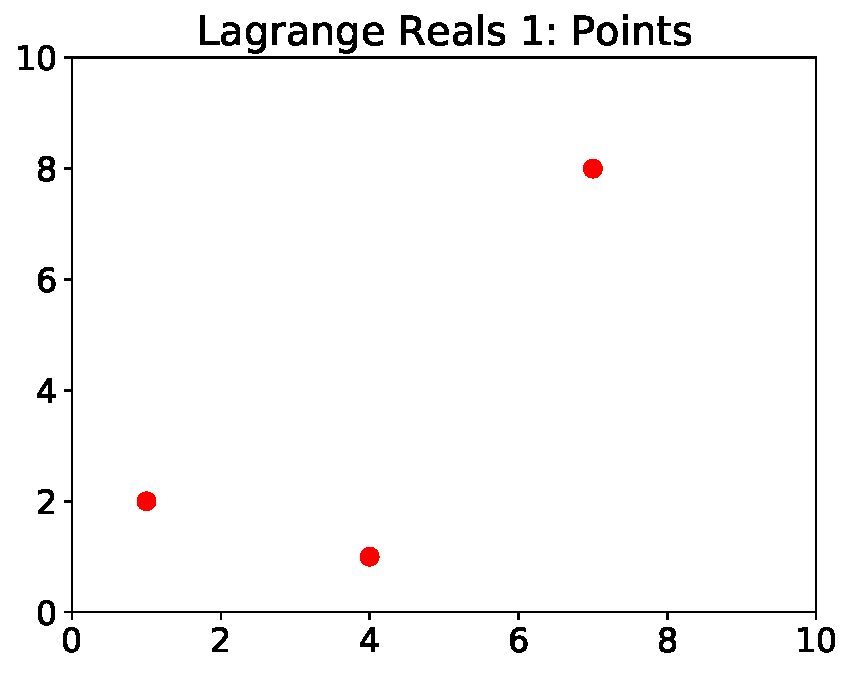
\includegraphics[width=\textwidth]{plots/lagrange/lagrange_reals_points_1.pdf}
    \caption{Lagrange interpolation data points}
    \label{fig:lagrange_points_1}
    \end{subfigure}
    \begin{subfigure}[t]{0.45\textwidth}
    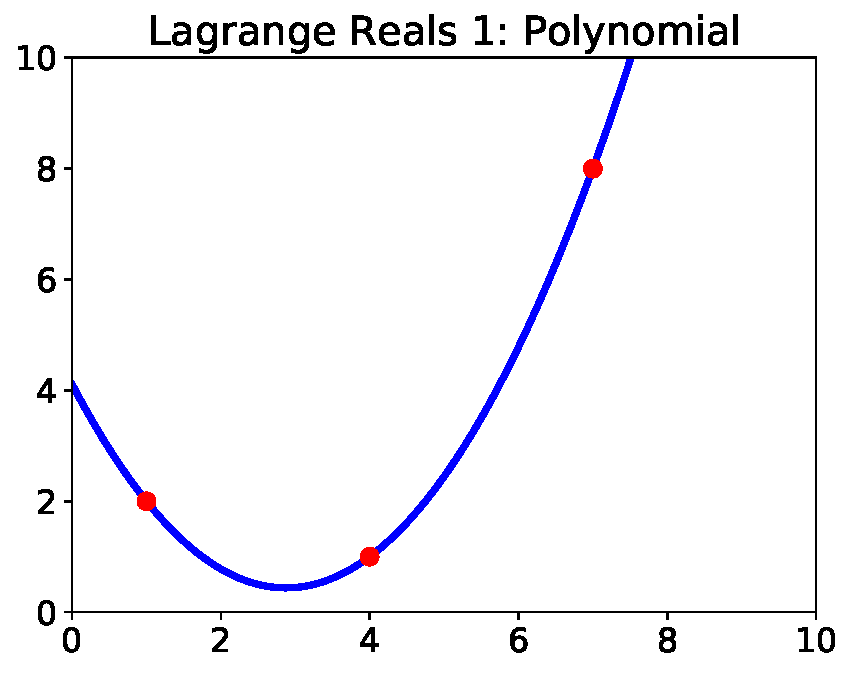
\includegraphics[width=\textwidth]{plots/lagrange/lagrange_reals_poly_1.pdf}
    \caption{Lagrange interpolation polynomial}
    \label{fig:lagrange_poly_1}
    \end{subfigure}
    \caption[Data points and Lagrange Interpolation over the reals 1]{Here
        are data points and Lagrange interpolating polynomial
        for Example~\ref{example:math_lagrange_reals_1}.}
\end{figure}



We start by computing the $\ell_{k}$ polynomials:

\begin{align}
    \ell_{1}(x) &= \frac{x-4}{1-4}\cdot\frac{x-7}{1-7}
        \nonumber\\
    \ell_{2}(x) &= \frac{x-1}{4-1}\cdot\frac{x-7}{4-7}
        \nonumber\\
    \ell_{3}(x) &= \frac{x-1}{7-1}\cdot\frac{x-4}{7-4}.
\end{align}

\noindent
In this case, we have the interpolating polynomial

\begin{equation}
    L(x) = 2\cdot\frac{x-4}{1-4}\cdot\frac{x-7}{1-7}
        + 1\cdot\frac{x-1}{4-1}\cdot\frac{x-7}{4-7}
        + 8\cdot\frac{x-1}{7-1}\cdot\frac{x-4}{7-4}.
\end{equation}

\noindent
This may be reduced to

\begin{equation}
    L(x) = \frac{1}{9}\brackets{4x^{2} - 23x + 37}.
\end{equation}

\noindent
The data points with this polynomial can be found in
Figure~\ref{fig:lagrange_poly_1}.
We see that

\begin{align}
    L(1) &= 2 \nonumber\\
    L(4) &= 1 \nonumber\\
    L(7) &= 8.
\end{align}
\end{example}

\begin{example}
\label{example:math_lagrange_reals_2}
\exampleCodeReference{examples/math\_review/lagrange\_reals\_2.py}

We interpolate the data
$\braces{\parens{1,2},\parens{4,1},\parens{5,1},\parens{7,8}}$;
this is the same data from the previous example with the additional
point $\parens{5,1}$.
See the data in Figure~\ref{fig:lagrange_points_2}.

\begin{figure}[t]
\centering
    \begin{subfigure}[t]{0.45\textwidth}
    \includegraphics[width=\textwidth]{plots/lagrange/lagrange_reals_points_2.pdf}
    \caption{Lagrange interpolation data points}
    \label{fig:lagrange_points_2}
    \end{subfigure}
    \begin{subfigure}[t]{0.45\textwidth}
    \includegraphics[width=\textwidth]{plots/lagrange/lagrange_reals_poly_2.pdf}
    \caption{Lagrange interpolation polynomial}
    \label{fig:lagrange_poly_2}
    \end{subfigure}
    \caption[Data points and Lagrange Interpolation over the reals 2]{Here
        are data points and Lagrange interpolating polynomial
        for Example~\ref{example:math_lagrange_reals_2}.}
\end{figure}



We again compute the $\ell_{k}$ polynomials:

\begin{align}
    \ell_{1}(x) &= \frac{x-4}{1-4}\cdot\frac{x-5}{1-5}\cdot\frac{x-7}{1-7}
        \nonumber\\
    \ell_{2}(x) &= \frac{x-1}{4-1}\cdot\frac{x-5}{4-5}\cdot\frac{x-7}{4-7}
        \nonumber\\
    \ell_{3}(x) &= \frac{x-1}{5-1}\cdot\frac{x-4}{5-4}\cdot\frac{x-7}{5-7}
        \nonumber\\
    \ell_{4}(x) &= \frac{x-1}{7-1}\cdot\frac{x-4}{7-4}\cdot\frac{x-5}{7-5}.
\end{align}

\noindent
The resulting Lagrange interpolation polynomial is

\begin{equation}
    L(x) = \frac{1}{72}\brackets{13x^{3} - 124x^{2} + 323x - 68}.
\end{equation}

\noindent
The data points with this polynomial can be found in
Figure~\ref{fig:lagrange_poly_2}.
\end{example}

\subsection{Problems with Lagrange Interpolation over the Reals}

We note that using \gls{lagrange interpolation} can lead to problems
when attempting to approximate certain types of \glspl{function} (data).
In particular, even with smooth functions
(functions with infinitely many derivatives),
it is possible that the polynomial approximation given by
\gls{lagrange interpolation} does not converge to the underlying function.
An example of this is shown in Figure~\ref{fig:math_lagrange_runge};
this is called \emph{Runge's Phenomenon}.

\begin{figure}[t]
\centering
    \includegraphics[width=10cm]{plots/lagrange/lagrange_runge.pdf}
    \caption[Plot of Runge's Phenomenon]{Here
        is an example of Runge's phenomenon.
        Even though the polynomial approximation of the \gls{function}
        $f(x) = \brackets{1+25x^{2}}^{-1}$
        is accurate close to $0$, the approximation is very poor
        near $1$ and $-1$.}
    \label{fig:math_lagrange_runge}
\end{figure}


There are mathematical reasons which can explain this,
but \emph{none} of those difficulties matter to us
because we are not particularly interested in interpolating
\glspl{function} over $\R$.
Rather, we are interested in interpolating polynomials over
\glspl{finite field}.

\subsection{Lagrange Interpolation over Finite Fields}

We are particularly interested in performing \gls{lagrange interpolation}
over \glspl{finite field}.
This will be used in secret sharing protocols.

There is effectively no difference between interpolation
over $\R$ and interpolation over $\F_{p}$.
This is because all of the operations in $\R$ directly translate
into the equivalent operations in $\F_{p}$.

\subsection{Examples of Lagrange Interpolation over Finite Fields}

We use the same examples as before except that now we use
the \gls{finite field} $\F_{73}$.



\begin{example}
\label{example:math_lagrange_finite_1}
\exampleCodeReference{examples/math\_review/lagrange\_finite\_1.py}

We begin by interpolating the data
$\braces{\parens{1,2},\parens{4,1},\parens{7,8}}$ as before
in Example~\ref{example:math_lagrange_reals_1};
in this case, we are interpolating over $\F_{73}$.
See the data in Figure~\ref{fig:lagrange_finite_points_1}.

\begin{figure}[t]
\centering
    \begin{subfigure}[t]{0.45\textwidth}
    \includegraphics[width=\textwidth]{plots/lagrange/lagrange_finite_points_1.pdf}
    \caption{Lagrange interpolation data points}
    \label{fig:lagrange_finite_points_1}
    \end{subfigure}
    \begin{subfigure}[t]{0.45\textwidth}
    \includegraphics[width=\textwidth]{plots/lagrange/lagrange_finite_poly_1.pdf}
    \caption{Lagrange interpolation polynomial}
    \label{fig:lagrange_finite_poly_1}
    \end{subfigure}
    \caption[Data points and Lagrange Interpolation over finite fields 1]{Here
        are data points and Lagrange interpolating polynomial
        for Example~\ref{example:math_lagrange_finite_1}.
        This example uses the \gls{finite field} $\F_{73}$.}
\end{figure}



In this case, we have the interpolating polynomial

\begin{equation}
    L(x) = 41x^{2} + 38x + 69.
\end{equation}

\noindent
The data points with this polynomial can be found in
Figure~\ref{fig:lagrange_finite_poly_1}.
We see that

\begin{align}
    L(1) &= 2 \nonumber\\
    L(4) &= 1 \nonumber\\
    L(7) &= 8.
\end{align}
\end{example}

\begin{example}
\label{example:math_lagrange_finite_2}
\exampleCodeReference{examples/math\_review/lagrange\_finite\_2.py}

We interpolate the data
$\braces{\parens{1,2},\parens{4,1},\parens{5,1},\parens{7,8}}$ as
in Example~\ref{example:math_lagrange_reals_2};
in this case, we are interpolating over $\F_{73}$.
See the data in Figure~\ref{fig:lagrange_finite_points_2}.

\begin{figure}[t]
\centering
    \begin{subfigure}[t]{0.45\textwidth}
    \includegraphics[width=\textwidth]{plots/lagrange/lagrange_finite_points_2.pdf}
    \caption{Lagrange interpolation data points}
    \label{fig:lagrange_finite_points_2}
    \end{subfigure}
    \begin{subfigure}[t]{0.45\textwidth}
    \includegraphics[width=\textwidth]{plots/lagrange/lagrange_finite_poly_2.pdf}
    \caption{Lagrange interpolation polynomial}
    \label{fig:lagrange_finite_poly_2}
    \end{subfigure}
    \caption[Data points and Lagrange Interpolation over finite fields 2]{Here
        are data points and Lagrange interpolating polynomial
        for Example~\ref{example:math_lagrange_finite_2}.
        This example uses the \gls{finite field} $\F_{73}$.}
\end{figure}



In this case, we have the interpolating polynomial

\begin{equation}
    L(x) = 60x^{3} + 51x^{2} + 42x + 68.
\end{equation}

\noindent
The data points with this polynomial can be found in
Figure~\ref{fig:lagrange_finite_poly_2}.
We see that

\begin{align}
    L(1) &= 2 \nonumber\\
    L(4) &= 1 \nonumber\\
    L(5) &= 1 \nonumber\\
    L(7) &= 8.
\end{align}
\end{example}

\subsection{Further Generalizations of Lagrange Interpolation}

It is possible to generalize \gls{lagrange interpolation} more.
In particular, by looking at Eq.~\eqref{eq:math_lagrange_def},
we see that all that is required of the data
$\braces{\parens{x_{i},y_{i}}}_{i=1}^{n}$
is that $\braces{x_{i}}$ must be elements of a \gls{field} $\F$
and $\braces{y_{i}}$ must be elements where it makes sense to perform
multiplication by $\F$.
Although this may appear to be an unnecessary generalization,
this will be used when computing threshold digital signatures
in Chapter~\ref{sec:ss_threshold};
in that setting, we are essentially interpolating over \gls{group} elements
parameterized by elements in a \gls{finite field}.


\section{Conclusion of Mathematical Review}

A lot of important and difficult material was covered
in the previous chapters.
There is still more mathematics that could be learned
and that would be useful for cryptography.
With that said, these are the main ideas and the most useful.
Studying additional mathematics would be recommended to anyone
who wants to dive deeper into cryptography;
see Chapter~\ref{chap:conclusion} for additional resources.
